\chapter{Appendix \autoref{chap:mad}}

\section{Implementation}
\label{app:implementation}

\begin{table}
\begin{center}
\begin{tabular}{c|c|c|c}
     Encoder $\Phi$ & Dense Layer & Mish & in\_size=$|\mathcal{X}|$, out\_size=$512$ \\
     & Dense Layer & Simnorm(8) & out\_size=$512$\\\hline
     
     & Dense Layer & Mish &in\_size=512 + $|\mathcal{A}|$, out\_size=$512$ \\
     Latent Model $F$ & Dense Layer & Mish & out\_size=$512$\\\
     & Dense Layer & Simnorm(8) &out\_size=$512$\\\hline
     
     & Dense Layer & Mish &in\_size=512 + $|\mathcal{A}|$, out\_size=$512$ \\
     Q head $\hat{Q}$& Dense Layer & Mish & out\_size=$512$\\
     & Dense Layer & -- & out\_size=$1$\\\hline

     & Dense Layer & Mish &in\_size=512, out\_size=$512$ \\
     Actor $\hat{\pi}$& Dense Layer & Mish & out\_size=$512$\\
     & Dense Layer & tanh & out\_size=$|\mathcal{A}|$
\end{tabular}
\end{center}
\caption{Network architecture for MAD-TD.}
\label{tab:arch}
\end{table}

\begin{table}
    \begin{tabular}{l|c}
        Parameter & \\\hline 
        Initial steps (Random policy) & $5000$  \\
        Batch size & $512$ \\
        RL learning rate & $0.0003$ \\
        Model learning rate & $0.0003$ \\
        Encoder learning rate & $0.0001$ \\
        Soft update $\tau$  & $0.995$ \\
        Discount factor $\gamma$  & $0.99$\\
        Model forward prediction steps & $1$ ($4$ for AR=1) \\
        Gradient clipping &  $10.0$ \\
        HL-Gauss vmin& $-150 \cdot \mathrm{AR}$ \\
    \end{tabular}
~
    \begin{tabular}{l|c}
        Parameter & \\\hline 
        HL-Gauss vmax& $150 \cdot \mathrm{AR}$\\ 
        HL-Gauss num bins& $151$\\
        Model data proportion& $0.95$\\
        Reset interval (where applicable)& $200000$\\
        Model \& encoder update ratio & $1$ \\
        Actor \& critic update ratio & varying \\
        MPC number of samples & $512$ \\
        MPC iterations& $6$ \\
        MPC top k& $64$\\
        MPC temperature& $0.5$
    \end{tabular}
    \caption{Hyperparameters. We adapted three parameters to the action repeat = 1 setting, as the magnitude of the reward changes.}
    \label{tab:hyperparams}
\end{table}

Our experiments are implemented in the jax library to allow for easy parallelization of multiple experiments across seeds.
All networks follow the standard architecture from \textcite{hansen2024tdmpc} with two changes: instead of using an ensemble of critics, we opt for a single double critic pair.
We also do not use a stochastic policy, instead simply using a deterministic network with a tanh activation as used in \textcite{ddpg,fujimoto2018addressing}.
Full hyperparameters are presented in \autoref{tab:hyperparams} and the architecture can be found in \autoref{tab:arch}.
We use mish activation functions \parencite{misra2020mish} and the adam optimizer to train our models \parencite{kingma2015adam}.

\paragraph{Loss functions:} As we use the HL-Gauss representation \parencite{farebrother2024stop} for the critic, the loss is the cross-entropy between the estimated Q function's categorical representation $Q_\mathrm{rep}$ and the bootstrapped TD estimate,
$$\mathcal{L}_Q = \sum_{i=1}^m {\mathrm{TD}(\hat{Q}_\mathrm{rep})}_i \log \hat{Q}_{\mathrm{rep}_i}\enspace,$$
where the indices $i$ denote the positions of the categorical vector representation used by HL-Gauss.
This is the same loss that is used for the two-hot encoding in \textcite{hansen2024tdmpc}, the only difference is the target encoding function.
For more details, see \textcite{farebrother2024stop}.

We use a latent encoder $\phi: \mathcal{X} \times \mathcal{A} \rightarrow \mathcal{Z}$ that maps into the simnorm space, the space of n k-dimensional simplicies \parencite{lavoie2023simplicial}.
Writing $\hat{p}$ for the learned world model and \mbox{$\hat{r}, \hat{x}' \sim \hat{p}(|x,a)$} for reward and next latent-state samples, the loss for our model and encoder is
\begin{align}
    \mathcal{L}_\mathrm{model}(x,a,r,x') &= \mathcal{L}_\mathrm{rew}(x,a,r) + \mathcal{L}_\mathrm{forward}(x,a,x') + \mathcal{L}_Q(x,a,r,x')\\
    \mathcal{L}_\mathrm{rew}(x,a,r) &= \left( r - \hat{r} \right)^2 \\
    \mathcal{L}_\mathrm{forward} &= - \sum_{i=1}^{n \cdot k} \phi(x')_i \log \hat{x}'_i\enspace,
\end{align}
where the index $i$ is again element-wise across the simplex representation used for the latent state.
Note that we propagate the critic learning gradients into the encoder only for the real data and not the model generated one to prevent instability.

\paragraph{Baseline results}
We took available results from \textcite{nauman2024bigger} and \textcite{hansen2024tdmpc} for all plots where possible, and used the official implementation of BRO to rerun the experiments without resetting and with differing action repeats. 
Other hyperparameters were left as-is.

\label{app:setup}

\newpage

\section{Further results}
\label{app:results}

\subsection{Q value overestimation}
\label{app:results_q}
\begin{figure}[ht]
    \centering
    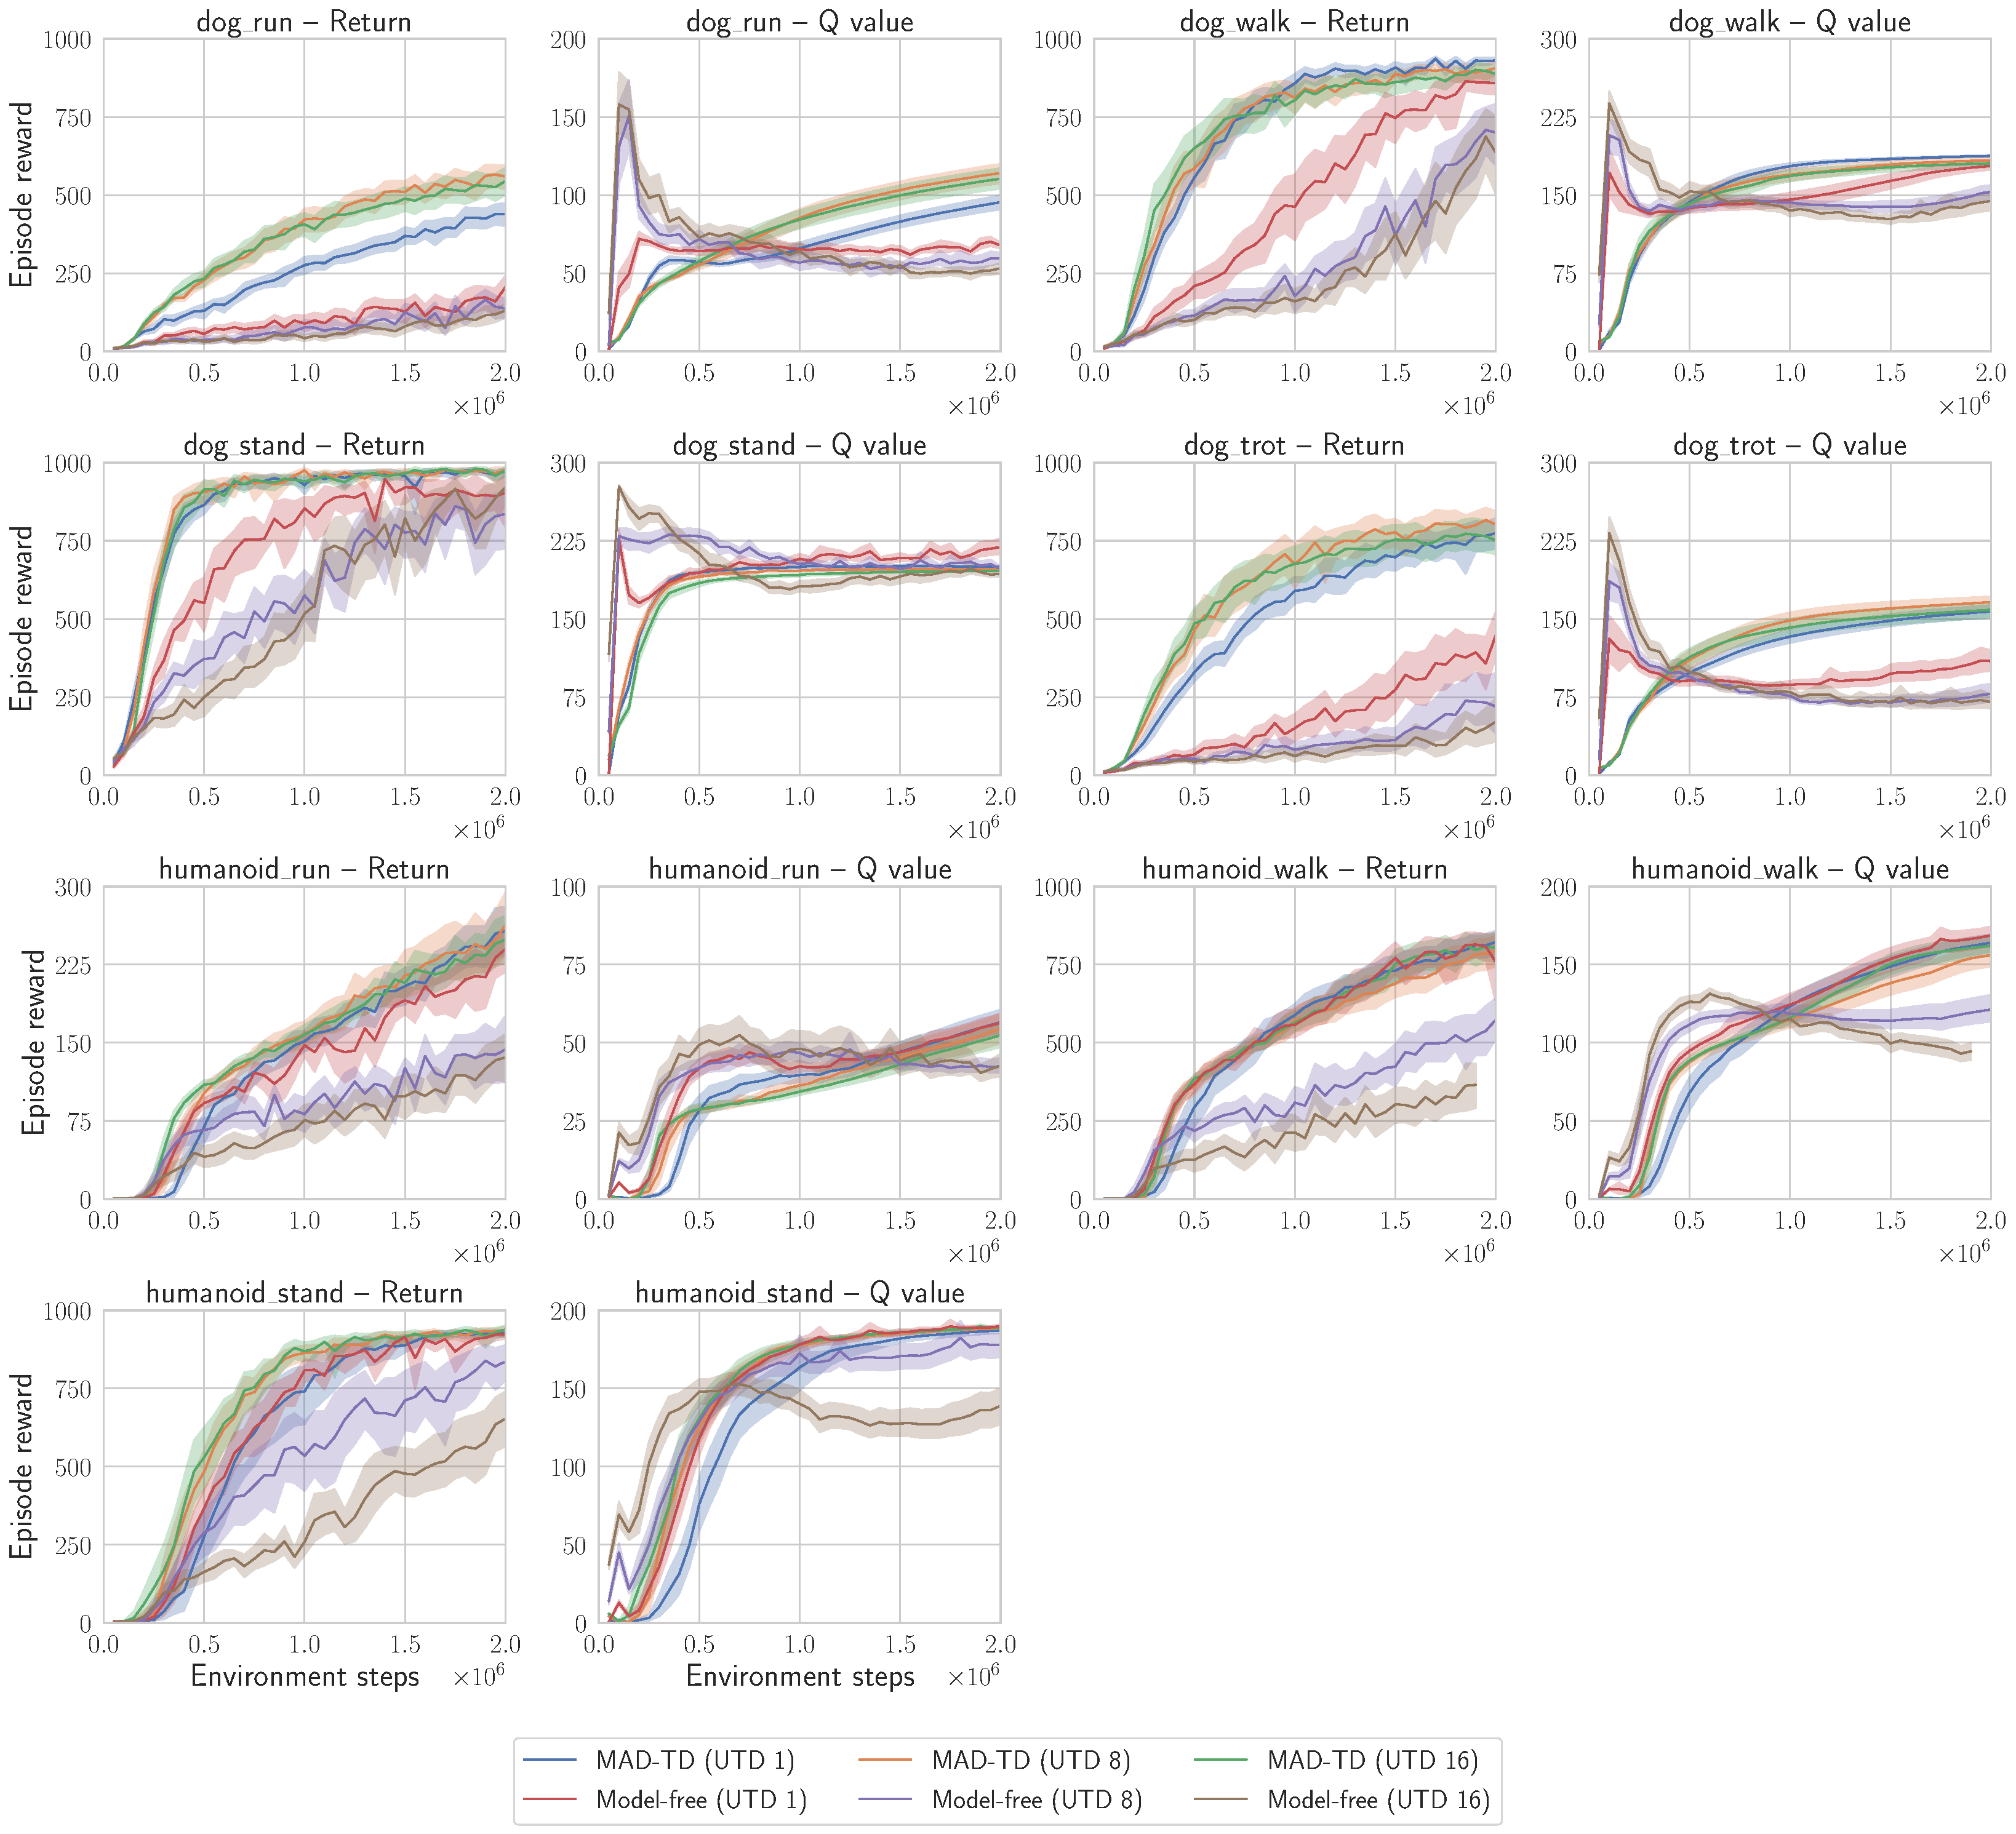
\includegraphics[width=\linewidth]{figures/mad-td/q_values_utd.pdf}
    \caption{Return curves and Q values with differing UTD values.}
    \label{fig:q_hard}
\end{figure}


We plot the return curves and corresponding Q estimates for different UTD values and with and without model-generated data on the hard suite.
The results are presented in \autoref{fig:q_hard}.
As we see, across all tasks the model free variant strongly overestimates the Q values, especially in the beginning.

\newpage

\subsection{Humanoid results}
\label{app:results_hum}


\begin{figure}[H]
    \centering
    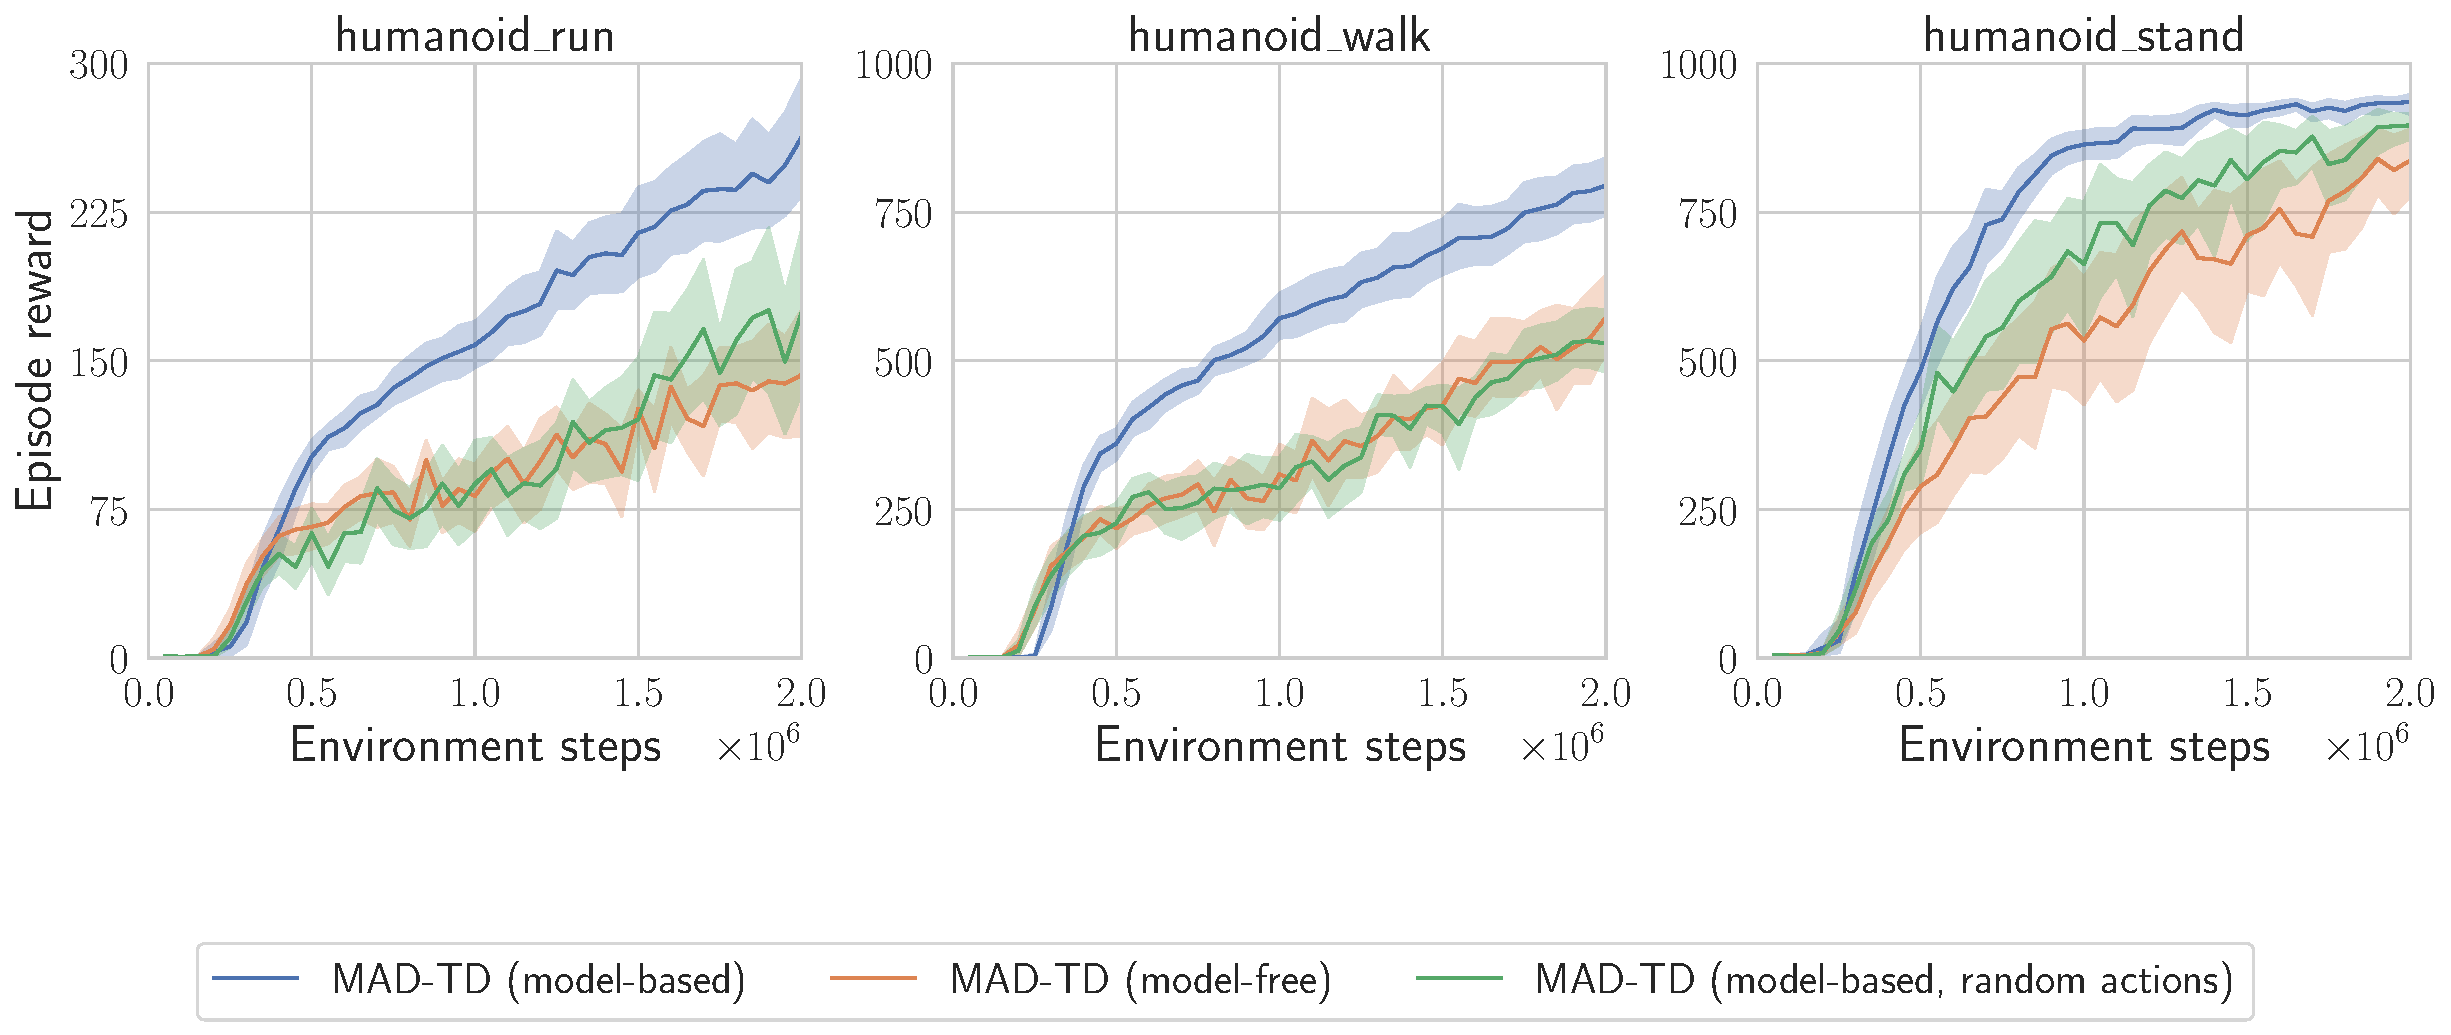
\includegraphics[width=0.9\linewidth]{figures/mad-td/humanoid_random_actions.pdf}
    \caption{Return curves for the humanoid tasks when using on-policy (blue), random (green) and no model-generated data (orange). The observed performance impacts are comparable to the dog case.}
    \label{fig:humanoid_random_actions}
\end{figure}

For several experiments, we only showed the dog results from the main suite to avoid cluttering the main body of the paper.
The corresponding humanoid results are presented in \autoref{fig:q_hard} and \autoref{fig:humanoid_random_actions}, corresponding to \autoref{fig:main_dog} and \autoref{fig:random_action} respectively.
As the plots highlight, the main insights transfer across the hard tasks.

\newpage

\subsection{Different quantities of model data}
\label{app:model_data}

We evaluate using more model data to update our value functions and provide the results in \autoref{fig:higher_data}.
\rebuttal{Aggregated scores are presented in \autoref{fig:higher_data_aggregate}.}
We observe that the majority of gain is obtained when using limited amount of model data, and larger amounts only provided limited gains in some humanoid runs.
\rebuttal{When using high amounts of model generated data, we observe deteriorating performance, which implies that the agent learns to exploit the model instead of solving the real task.
This observation is consistent with similar observation about model exploration in prior work \textcite{zhao2023simplified}}.

\begin{figure}[H]
    \centering
    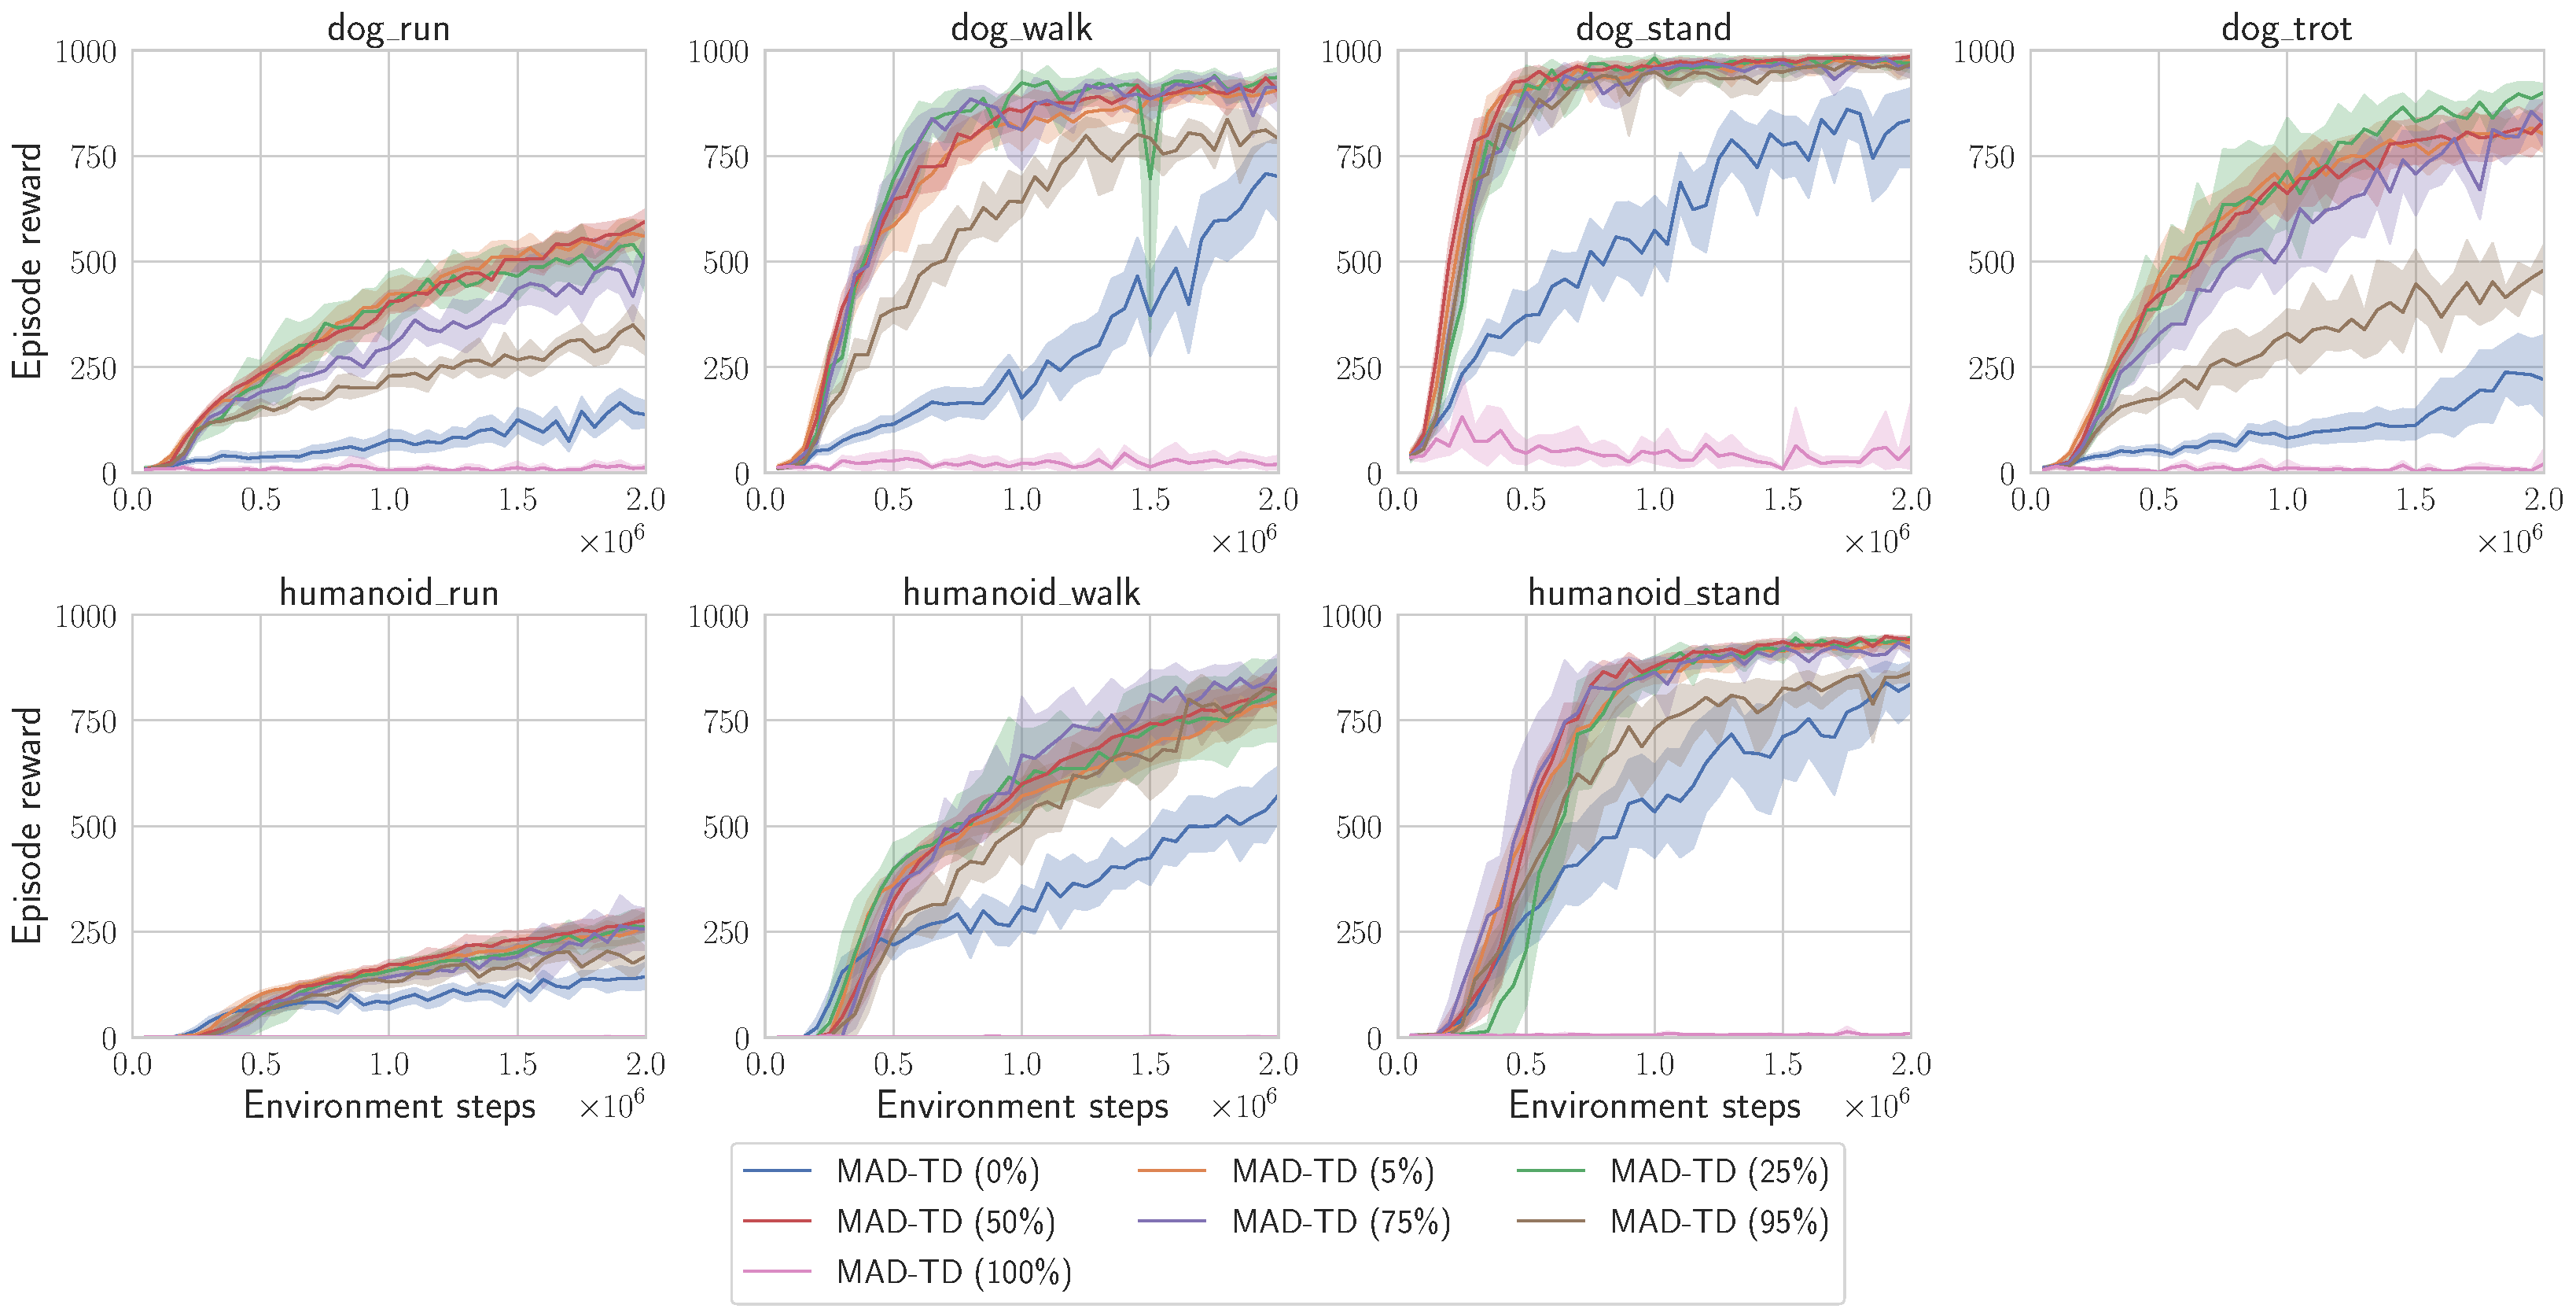
\includegraphics[width=\linewidth]{figures/mad-td/higher_data.pdf}
    \caption{Return curves on the hard suite. We see that using substantially more data than 5\% does not improve performance in a statistically significant way.}
    \label{fig:higher_data}
\end{figure}

\begin{figure}[H]
    \centering
    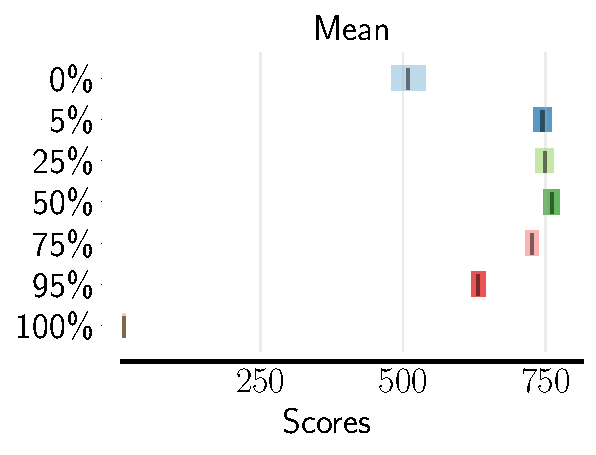
\includegraphics[width=0.4\linewidth]{figures/mad-td/higher_data_aggregate.pdf}
    \caption{Aggregate statistics for differing values of $\alpha$ (amount of model data used) at UTD 8.}
    \label{fig:higher_data_aggregate}
\end{figure}

\newpage

\rebuttal{
\subsection{SynthER comparison}
\label{app:synther}

We present a comparison of our method and SynthER on the hard DMC tasks.
Results can be found in \autoref{fig:synther}.

As is evident from the lack of strong performance of SynthER, merely increasing the amount of generated data is insufficient to combat the failure of learning at high UTD.
We find that the Q values of the SynthER agents quickly diverge on all tasks in which it is unable to learn.
This strengthens our hypothesis that for hard tasks, off-policy action correction is vital to achieve strong results.
}

\begin{figure}[H]
    \centering
    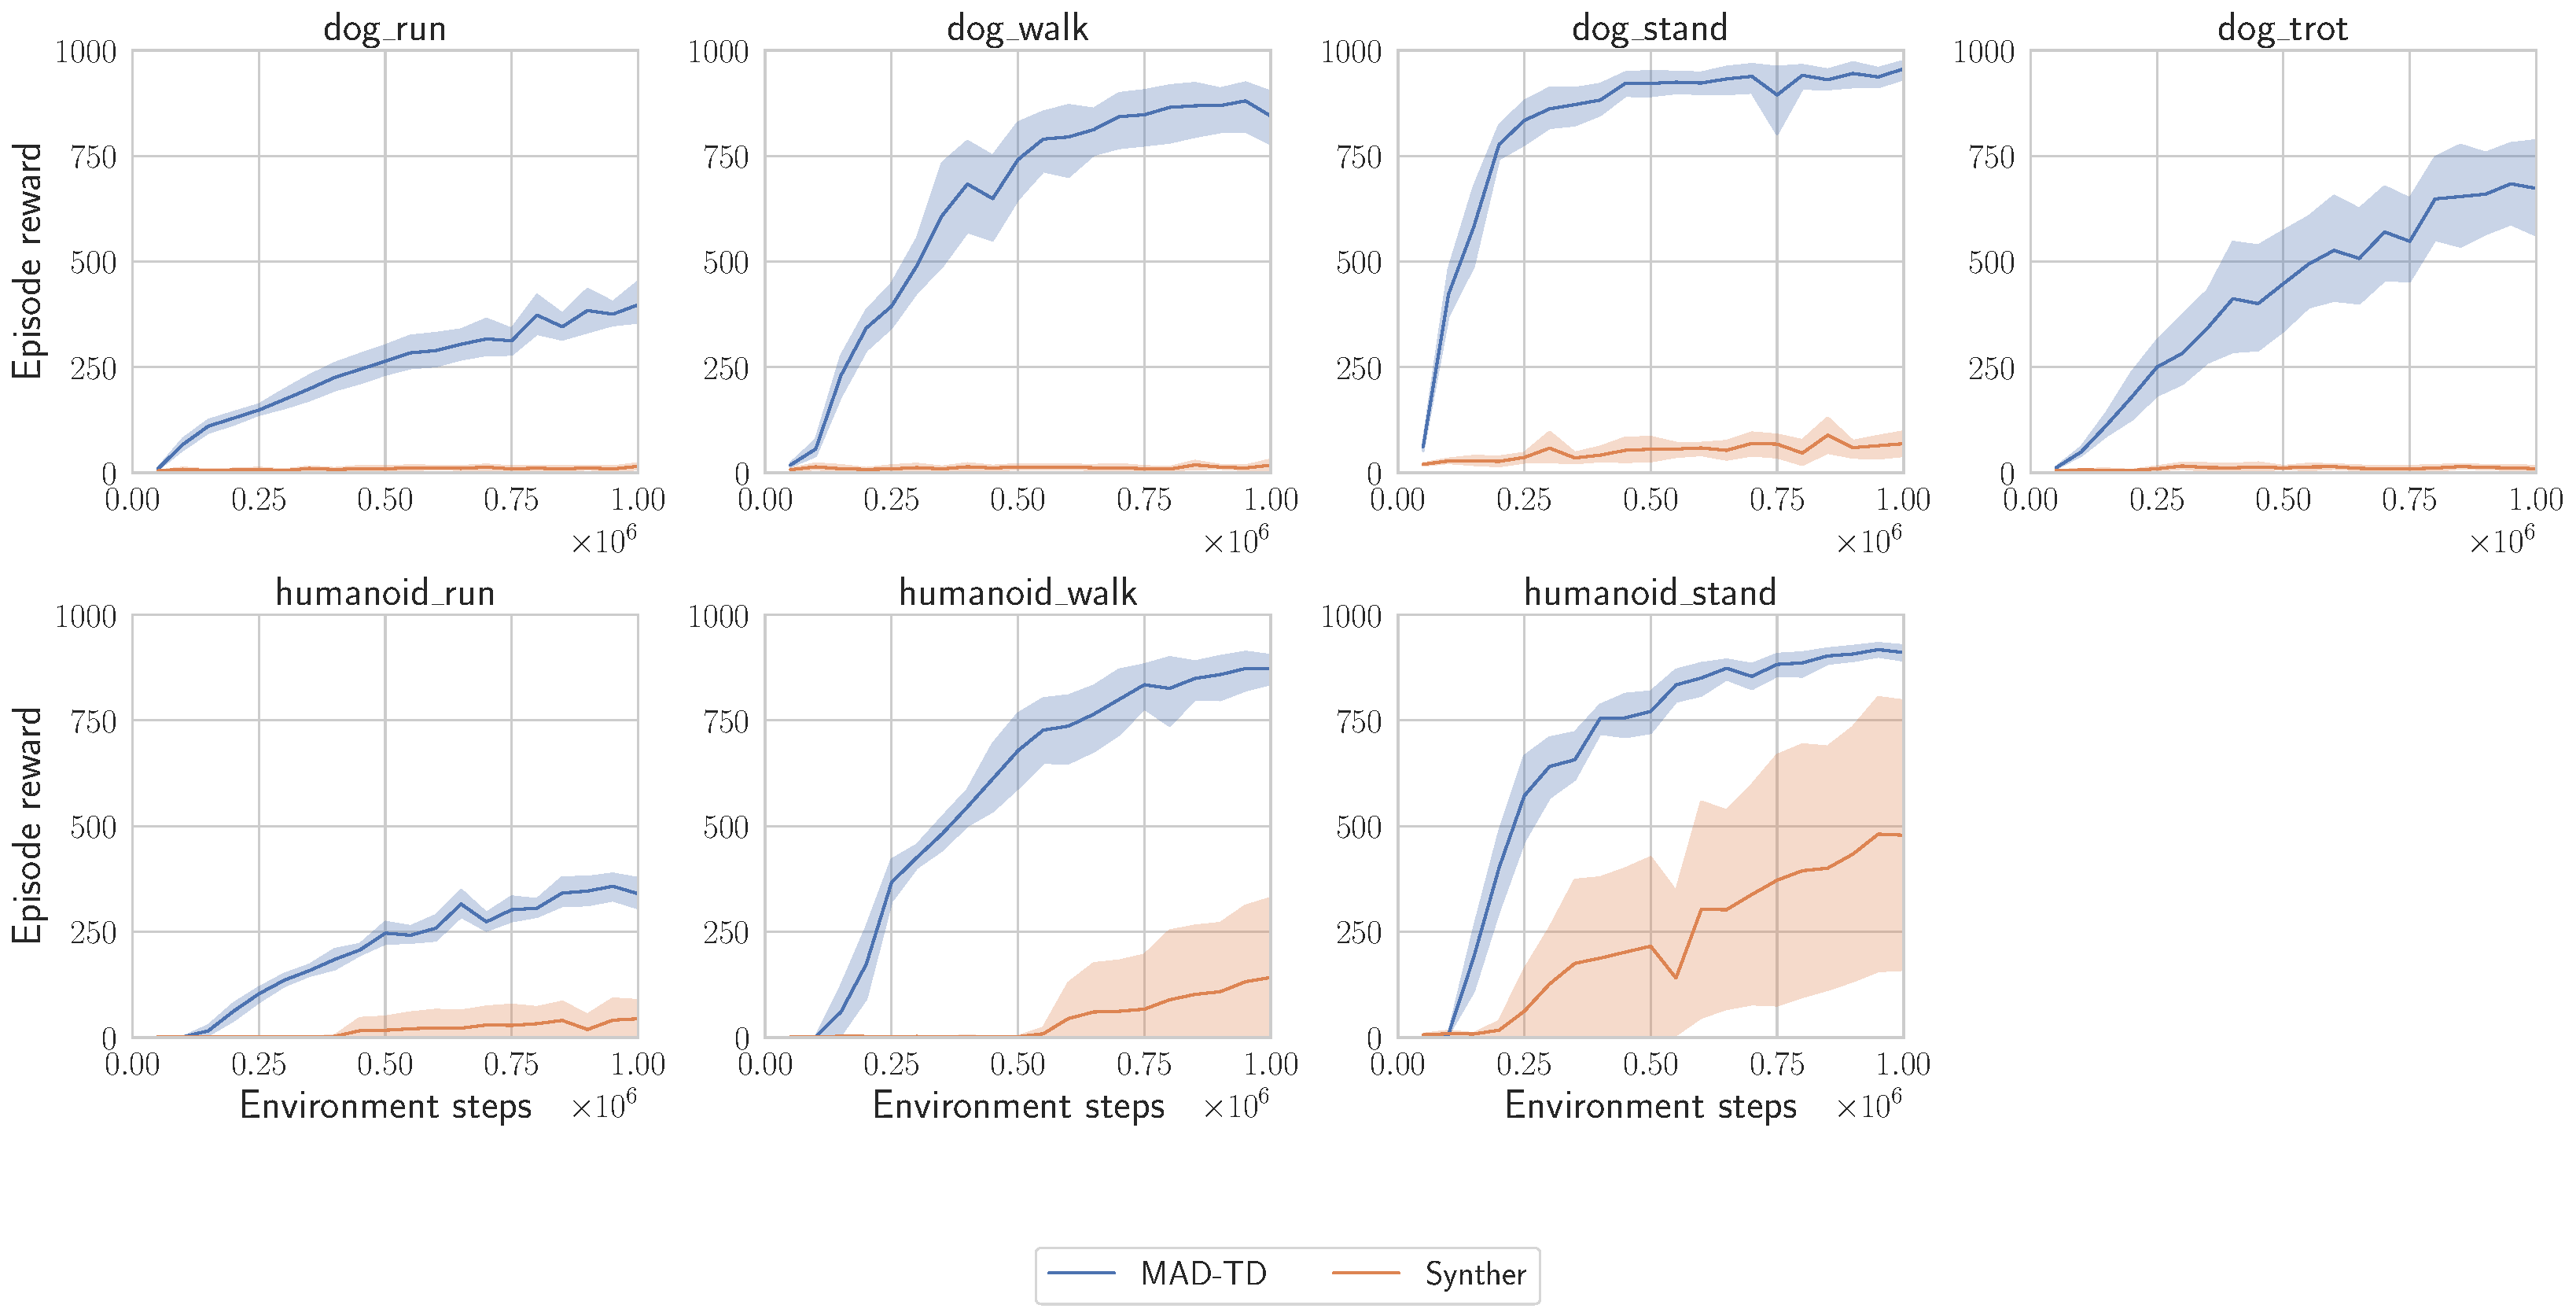
\includegraphics[width=\linewidth]{figures/mad-td/hard_fs_1_synther.pdf}
    \caption{\rebuttal{Performance curves for MAD-TD and SynthER on the hard DMC tasks. SynthER fails to achieve nontrivial results on most tasks, only outperforming a random policy on the humanoid walk and stand tasks. }}
    \label{fig:synther}
\end{figure}

\newpage

\rebuttal{
\subsection{TD-MPC2 ablation}
\label{app:ablation}

As described in the main paper, we simplify the base model of TD-MPC2 to improve the computational efficiency of the algorithm.
This is necessary to conduct high UTD experiments.
Here, we present a direct comparison of the original TD-MPC2 model, and our adapted version (\autoref{fig:tdmpc_ablation}).
We compare MAD-TD without any model generated data, at UTD 1, which corresponds to the standard setting of TD-MPC2.
As pointed out in the main paper, all of our changes to the base model boil down to setting different hyperparameters, such as the rollout length, to achieve faster learning.

We find that this does not significantly change the overall results achieved by the base model, and we are therefore confident to attribute performance gains to our presented method.
}

\begin{figure}[H]
    \centering
    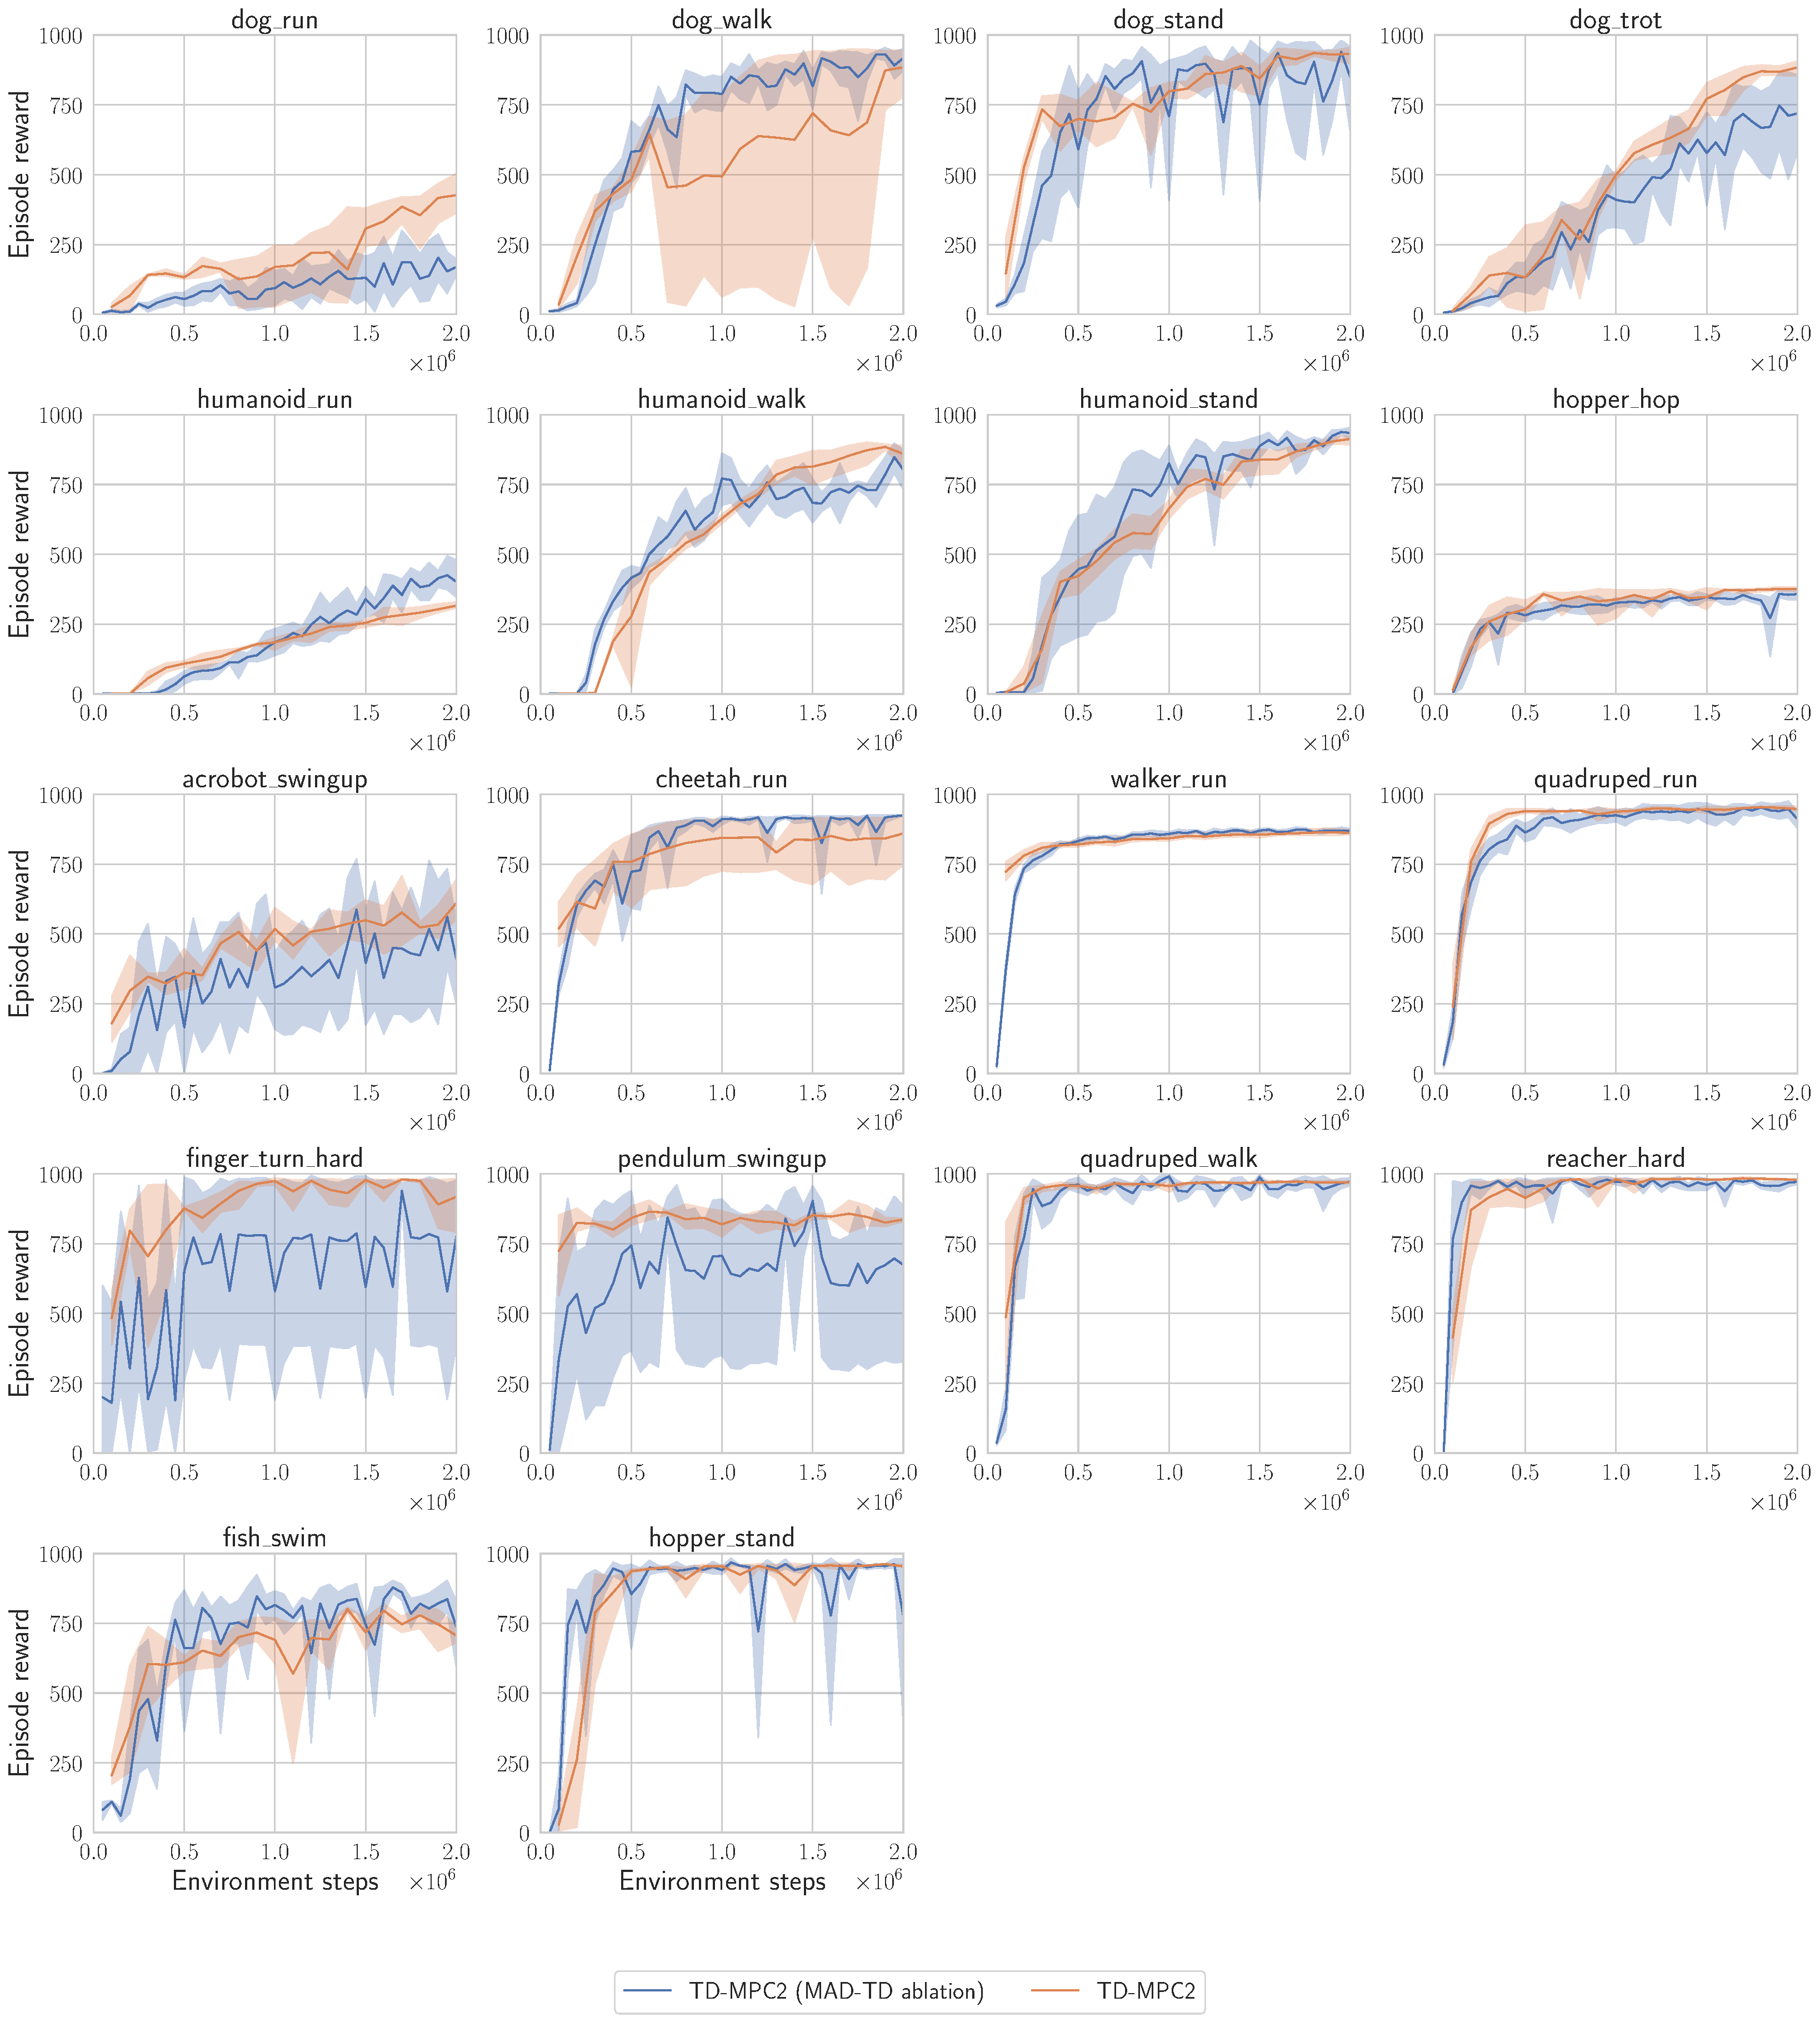
\includegraphics[width=\linewidth]{figures/mad-td/ablation.pdf}
    \caption{\rebuttal{Performance variation of the base MAD-TD model compared to TD-MPC2. Our changes only very few times lead to lower performance which is acceptable given the large reduction in computational cost.}}
    \label{fig:tdmpc_ablation}
\end{figure}

\newpage

\subsection{MAD-TD, BRO, TD-MPC2 per env on the hard suite}
\label{app:results_base}

We present the return curves for MAD-TD and the baselines per environment on the hard suite.
\autoref{fig:hard_all_fs_2} shows the results with action repeat 2 and \autoref{fig:hard_all_fs_1} with action repeat 1. 
Perhaps surprisingly, the results of the algorithms are not fully consistent across this regime. 
Partially, this can be explained by the fact that our method and TD-MPC2 were first developed in the regime of action repeat 2, while BRO was only evaluated in the action repeat 1 setting.
This suggests that the performance of each method depends in a non-trivial fashion on hyperparameter tuning.
Yet, across both action repeat setting MAD-TD outperforms BRO without resetting consistently and only under-performs any previous algorithm on the dog trot task in the action repeat 1 setting.

\begin{figure}[H]
    \centering
    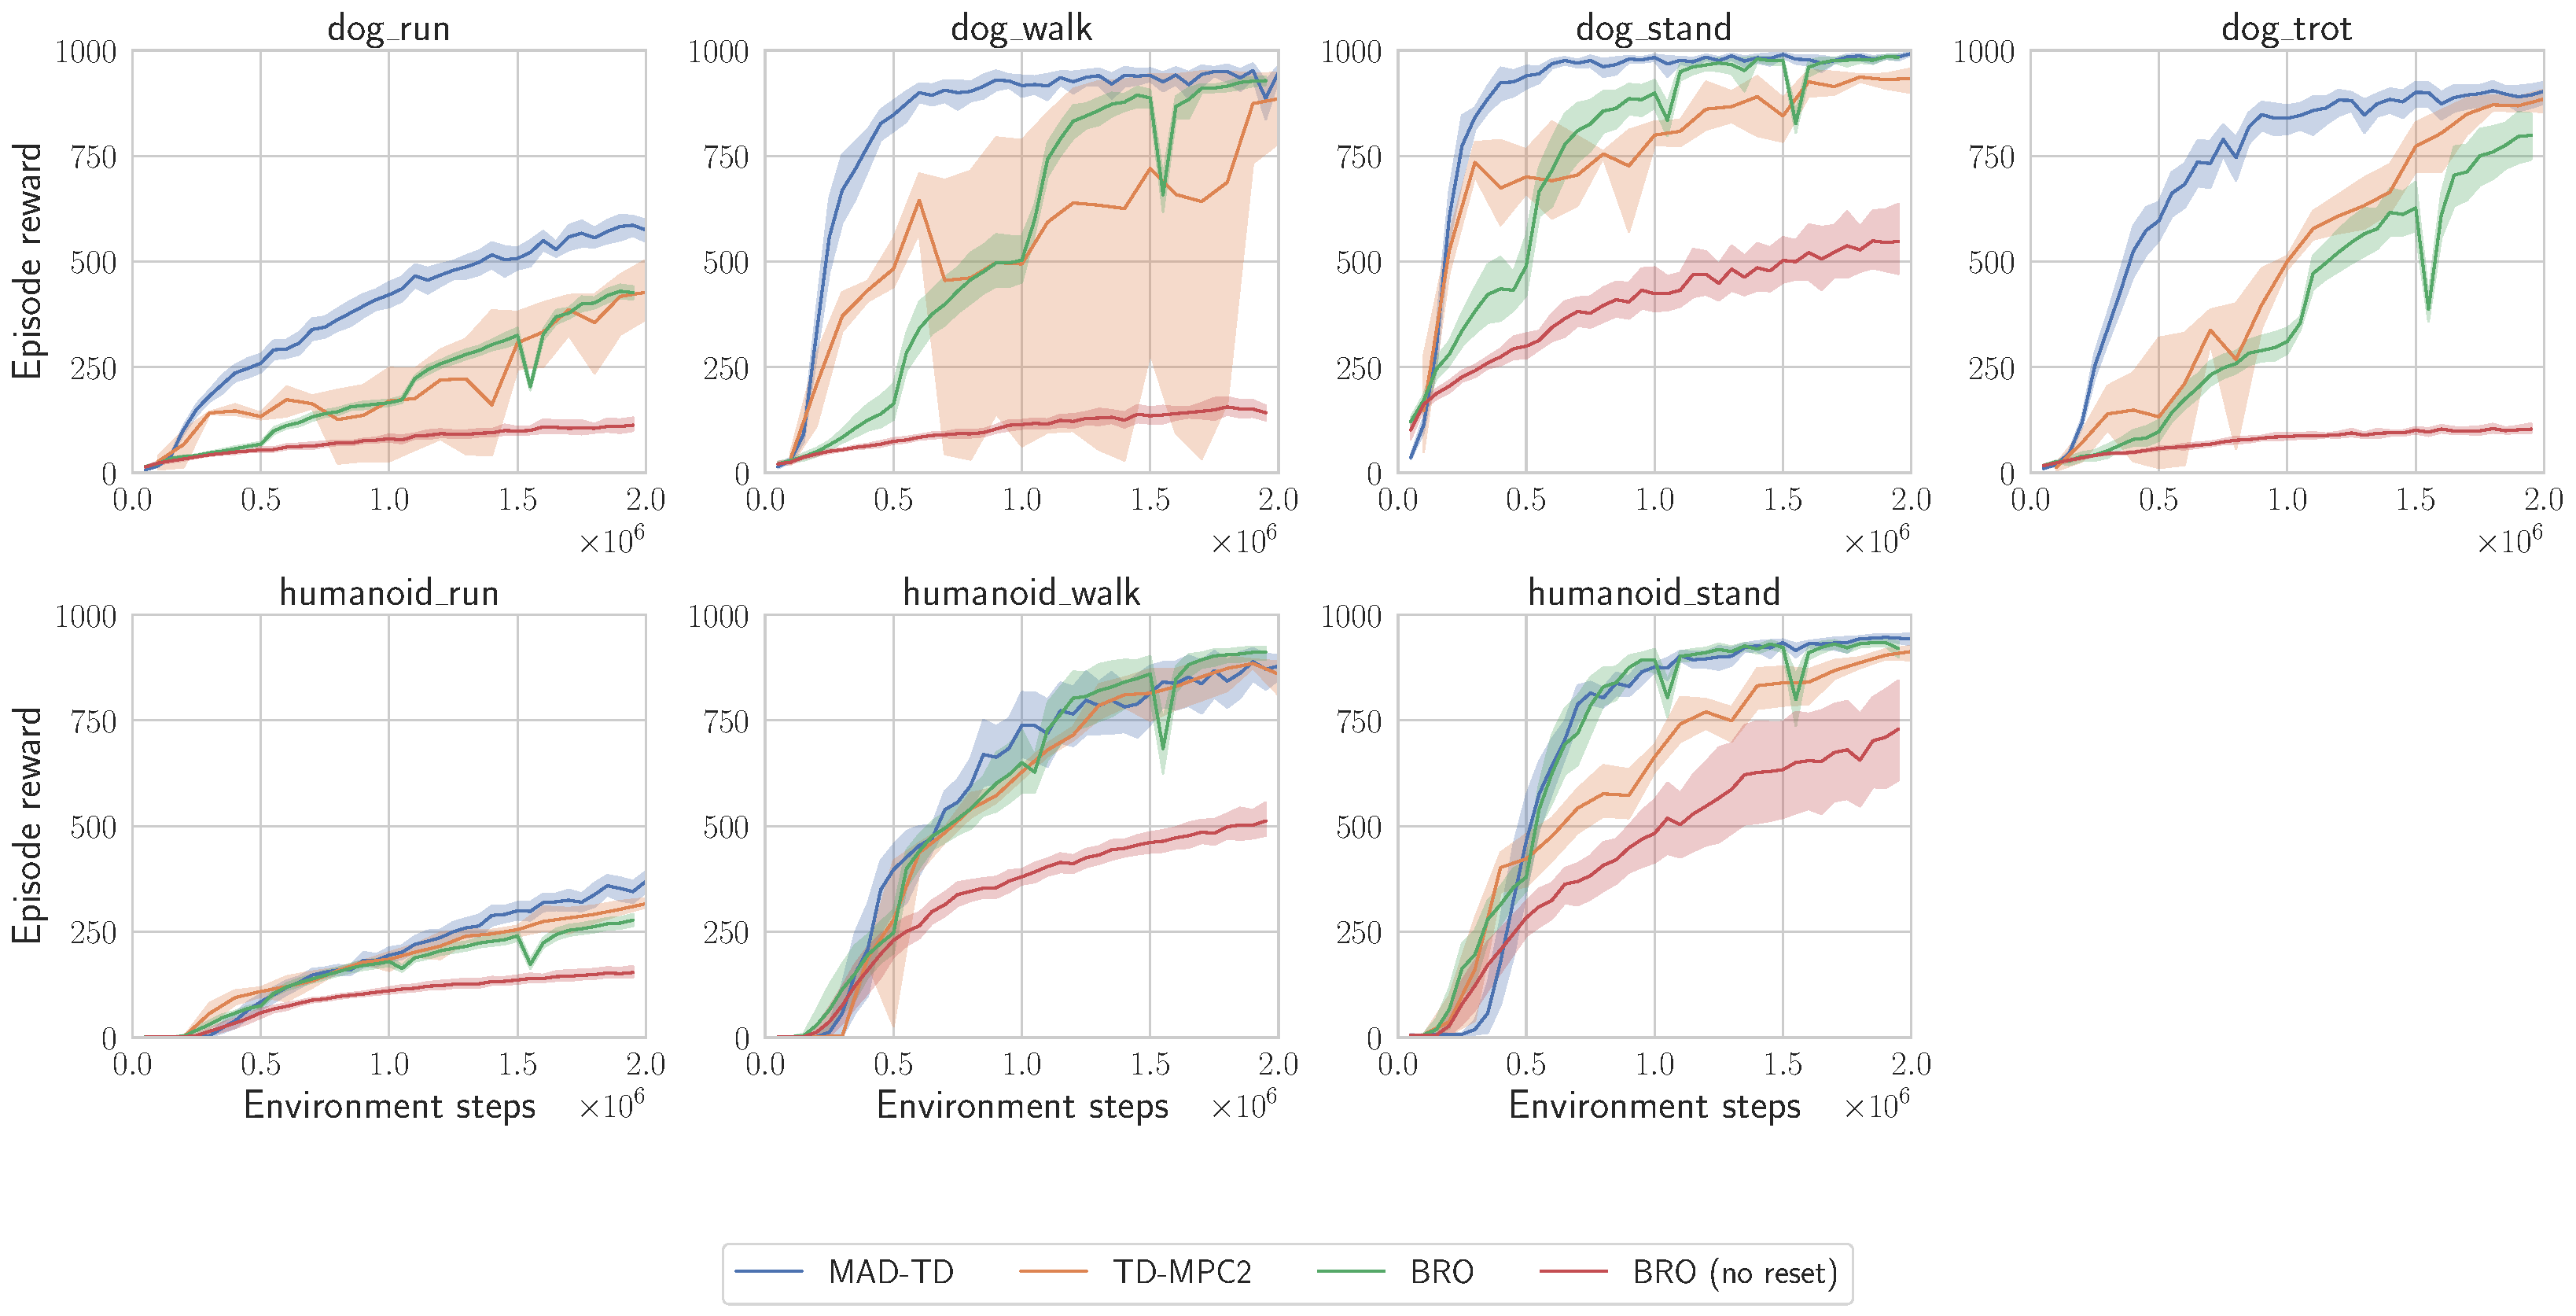
\includegraphics[width=0.8\linewidth]{figures/mad-td/hard_all_fs_2.pdf}
    \caption{Return curves with action repeat set to 2.}
    \label{fig:hard_all_fs_2}
\end{figure}

\begin{figure}[H]
    \centering
    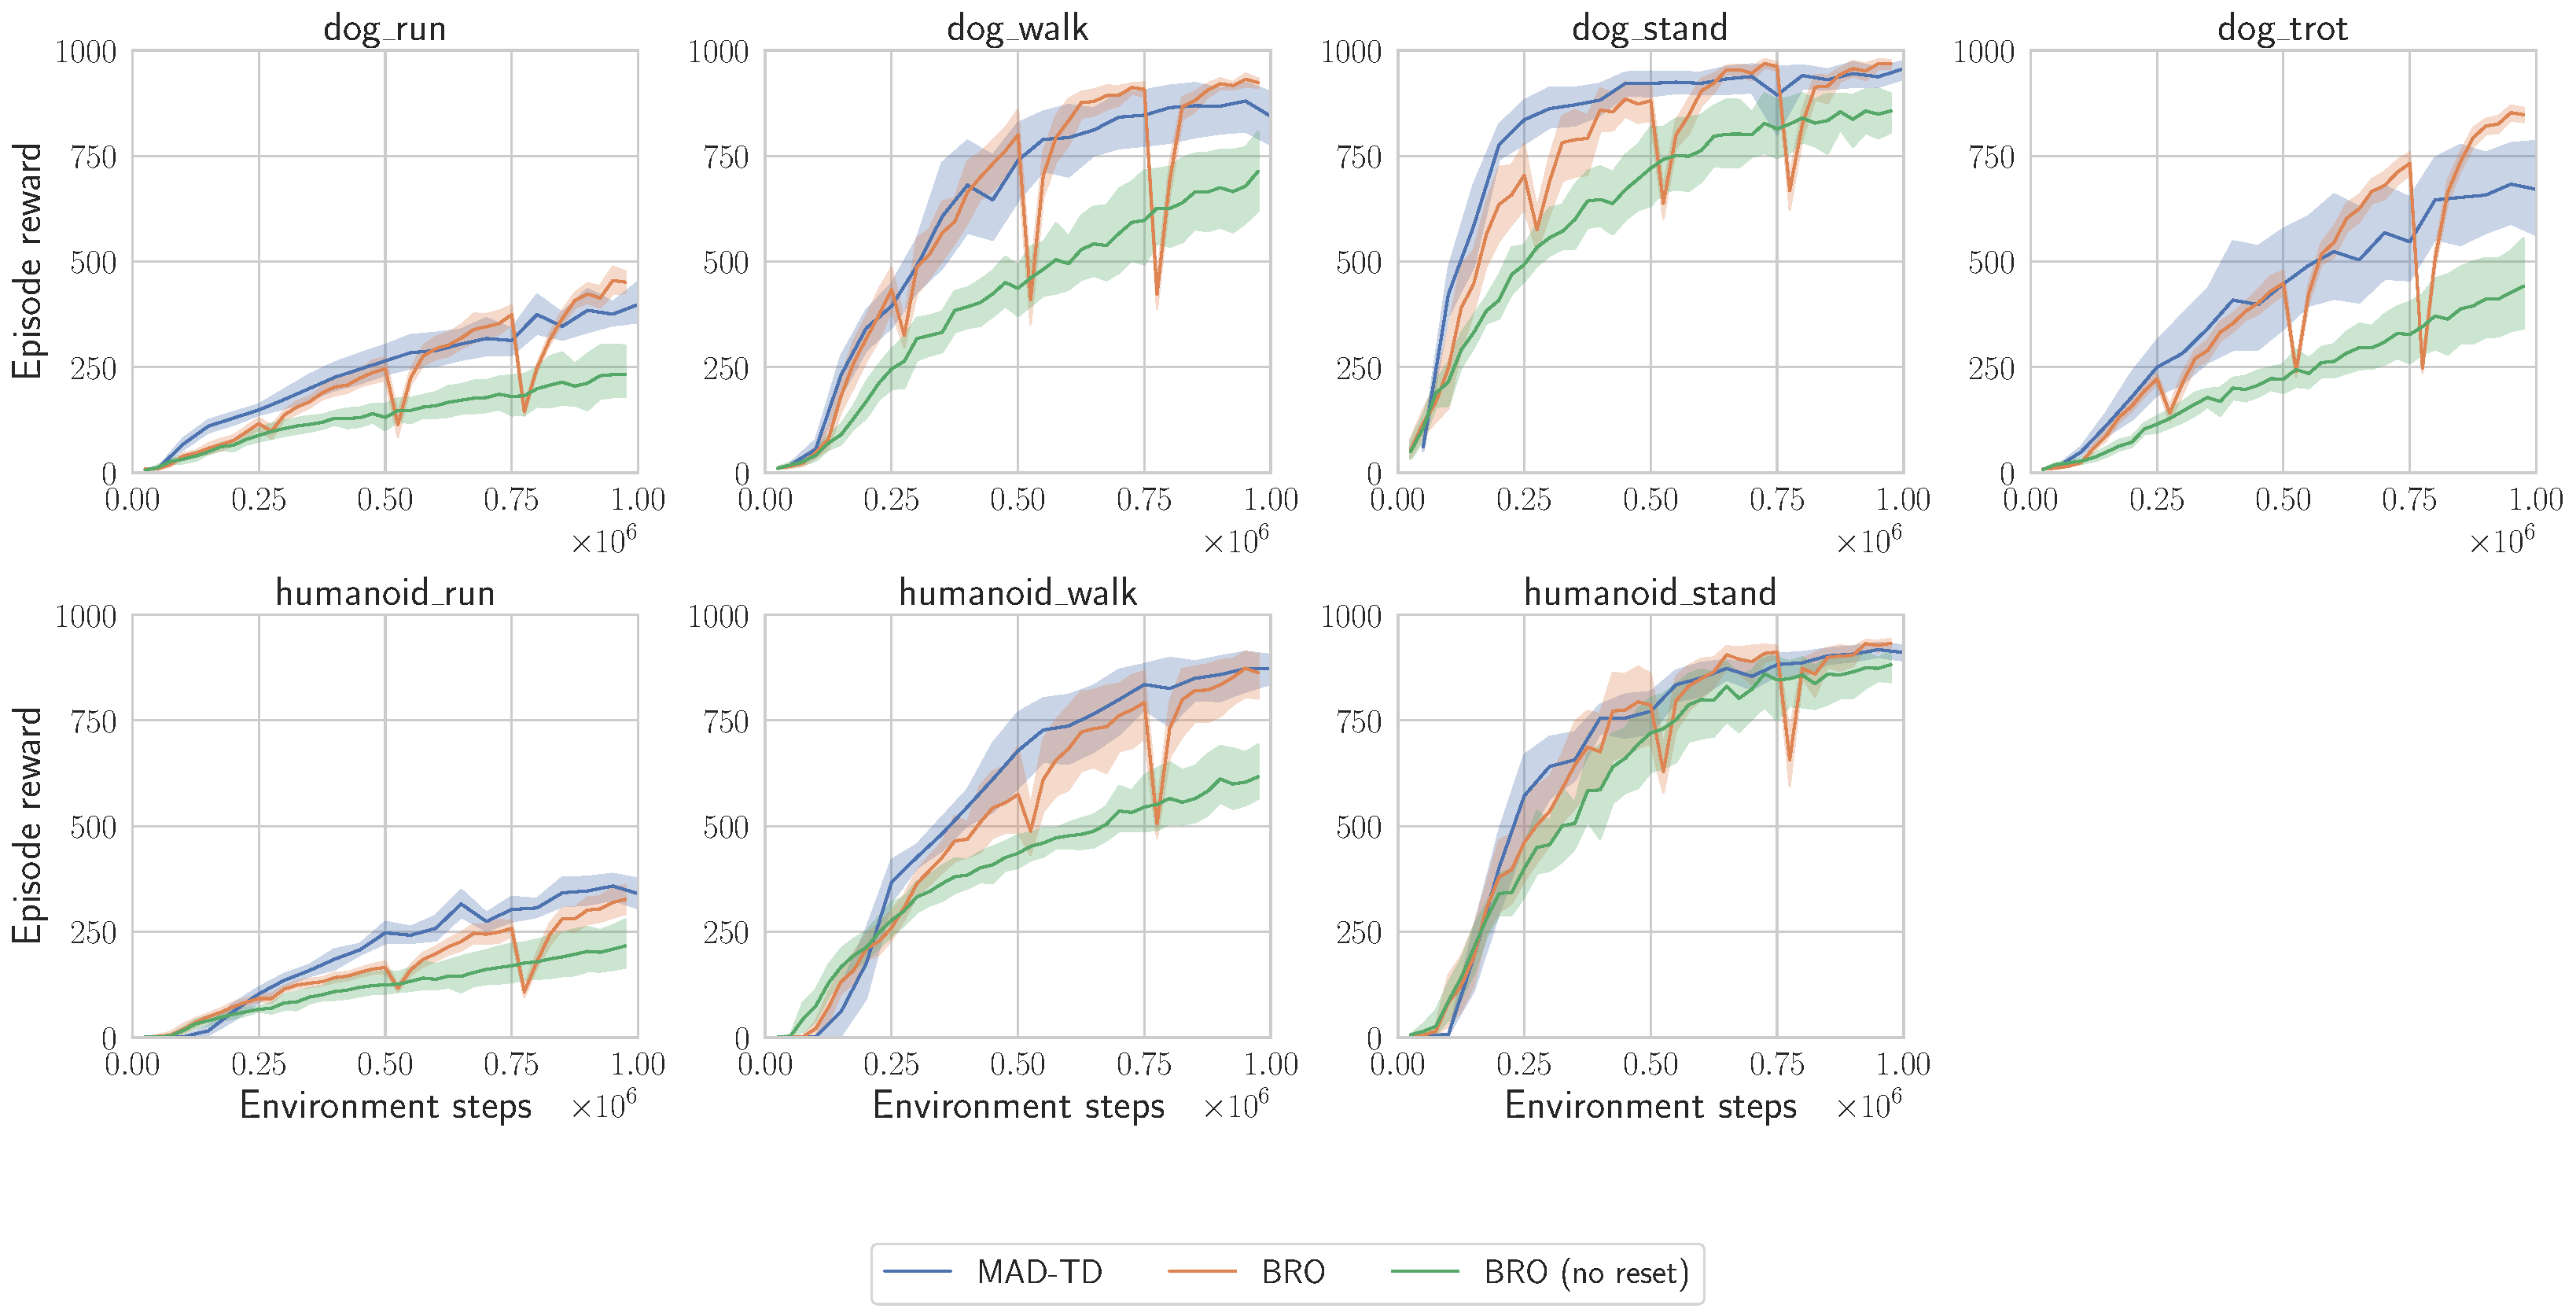
\includegraphics[width=0.8\linewidth]{figures/mad-td/hard_all_fs_1.pdf}
    \caption{Return curves with action repeat set to 1.}
    \label{fig:hard_all_fs_1}
\end{figure}

We conjecture that the remaining gap in performance seems to be most likely attributable to exploration and optimism.
While we focus on learning accurate value functions, Bro contains several components which are specifically designed to improve exploration.
Investigating the tension between exploration and accurate value function fitting is an important direction for future work.

Bro and TD-MPC2 are explicitly evaluated without their exploration bonuses in separate evaluation rollouts.
We however do not conduct such as separate evaluation as we do not add any additional exploration noise to our training.
When plotting training performance, the gap between MAD-TD and Bro further closes, suggesting an important trade-off between test time and training performance.

\subsection{Results across further DMC environments}
\label{app:results_further}

We conducted more experiments on all DMC environments which were shown to benefit from the interventions in prior work \parencite{doro2023barrier,nauman2024bigger}.

\begin{figure}[h]
    \centering
    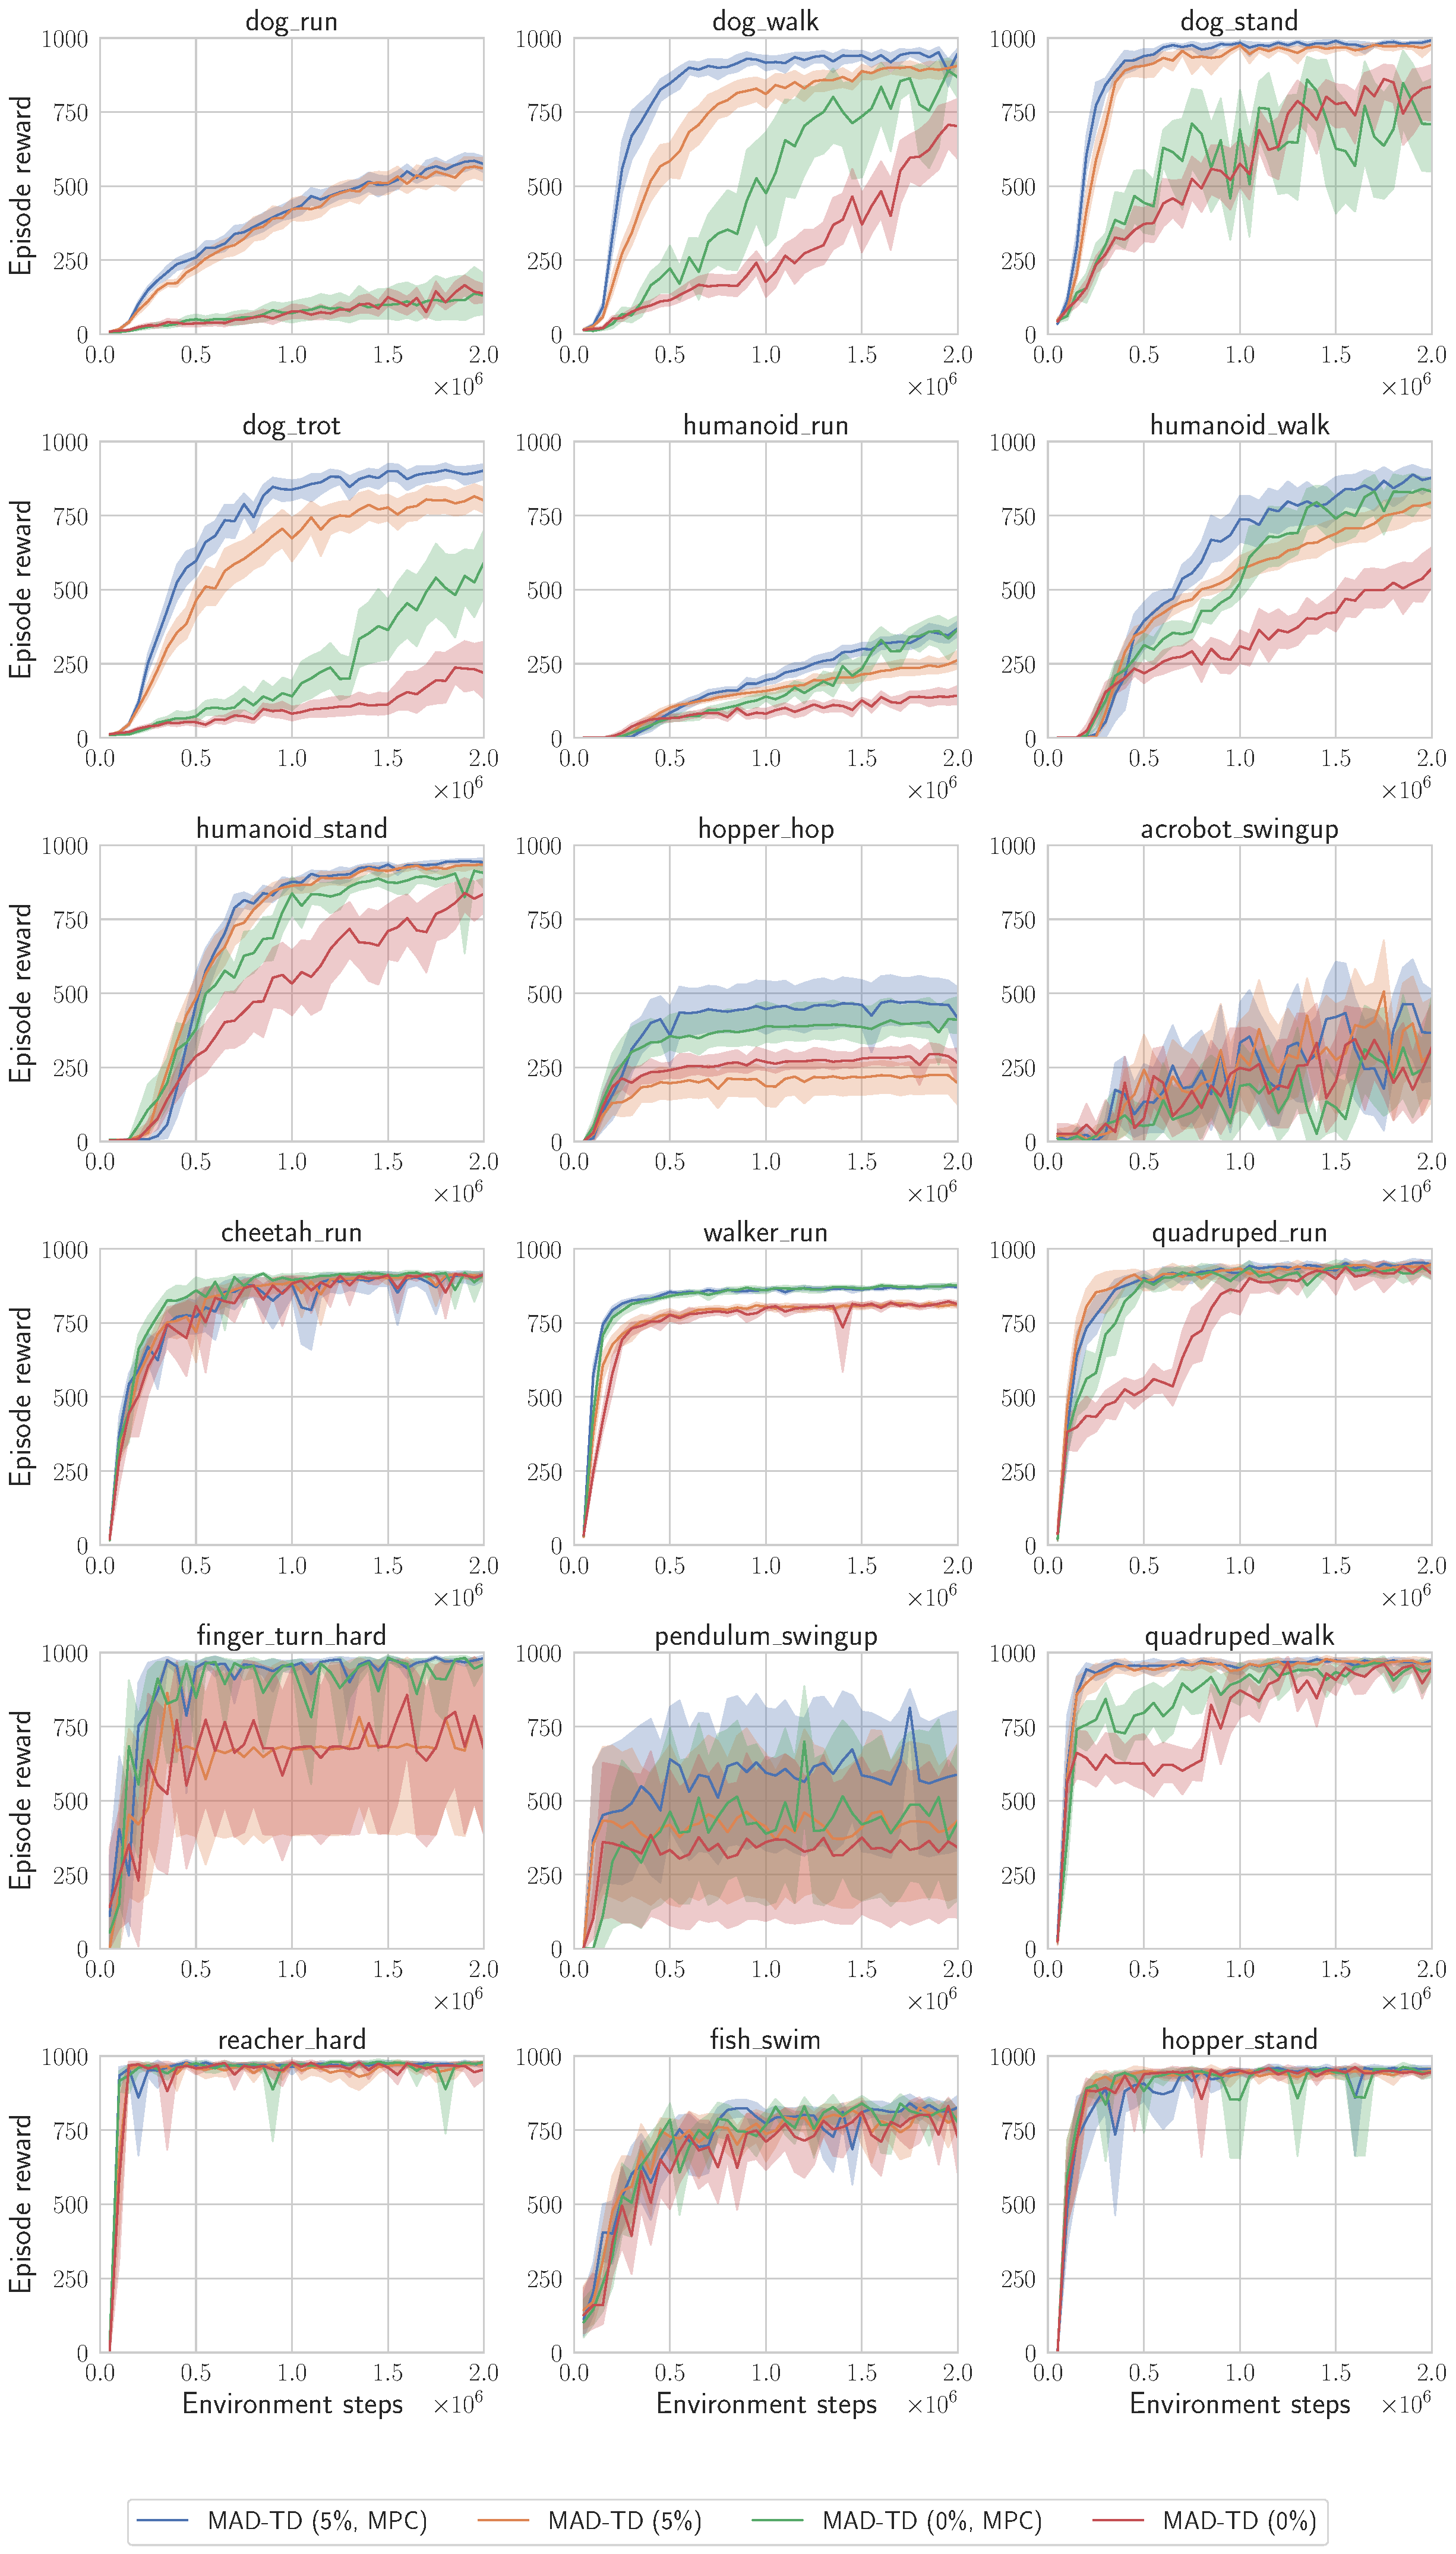
\includegraphics[width=0.8\linewidth]{figures/mad-td/model_impact.pdf}
    \caption{Return curves evaluating the impact of model-based data for critic learning and MPC. Overall, MPC and model-based critic learning both stabilize the learning process, as conjectured.}
    \label{fig:all_model_impact}
\end{figure}

\begin{figure}[H]
    \centering
    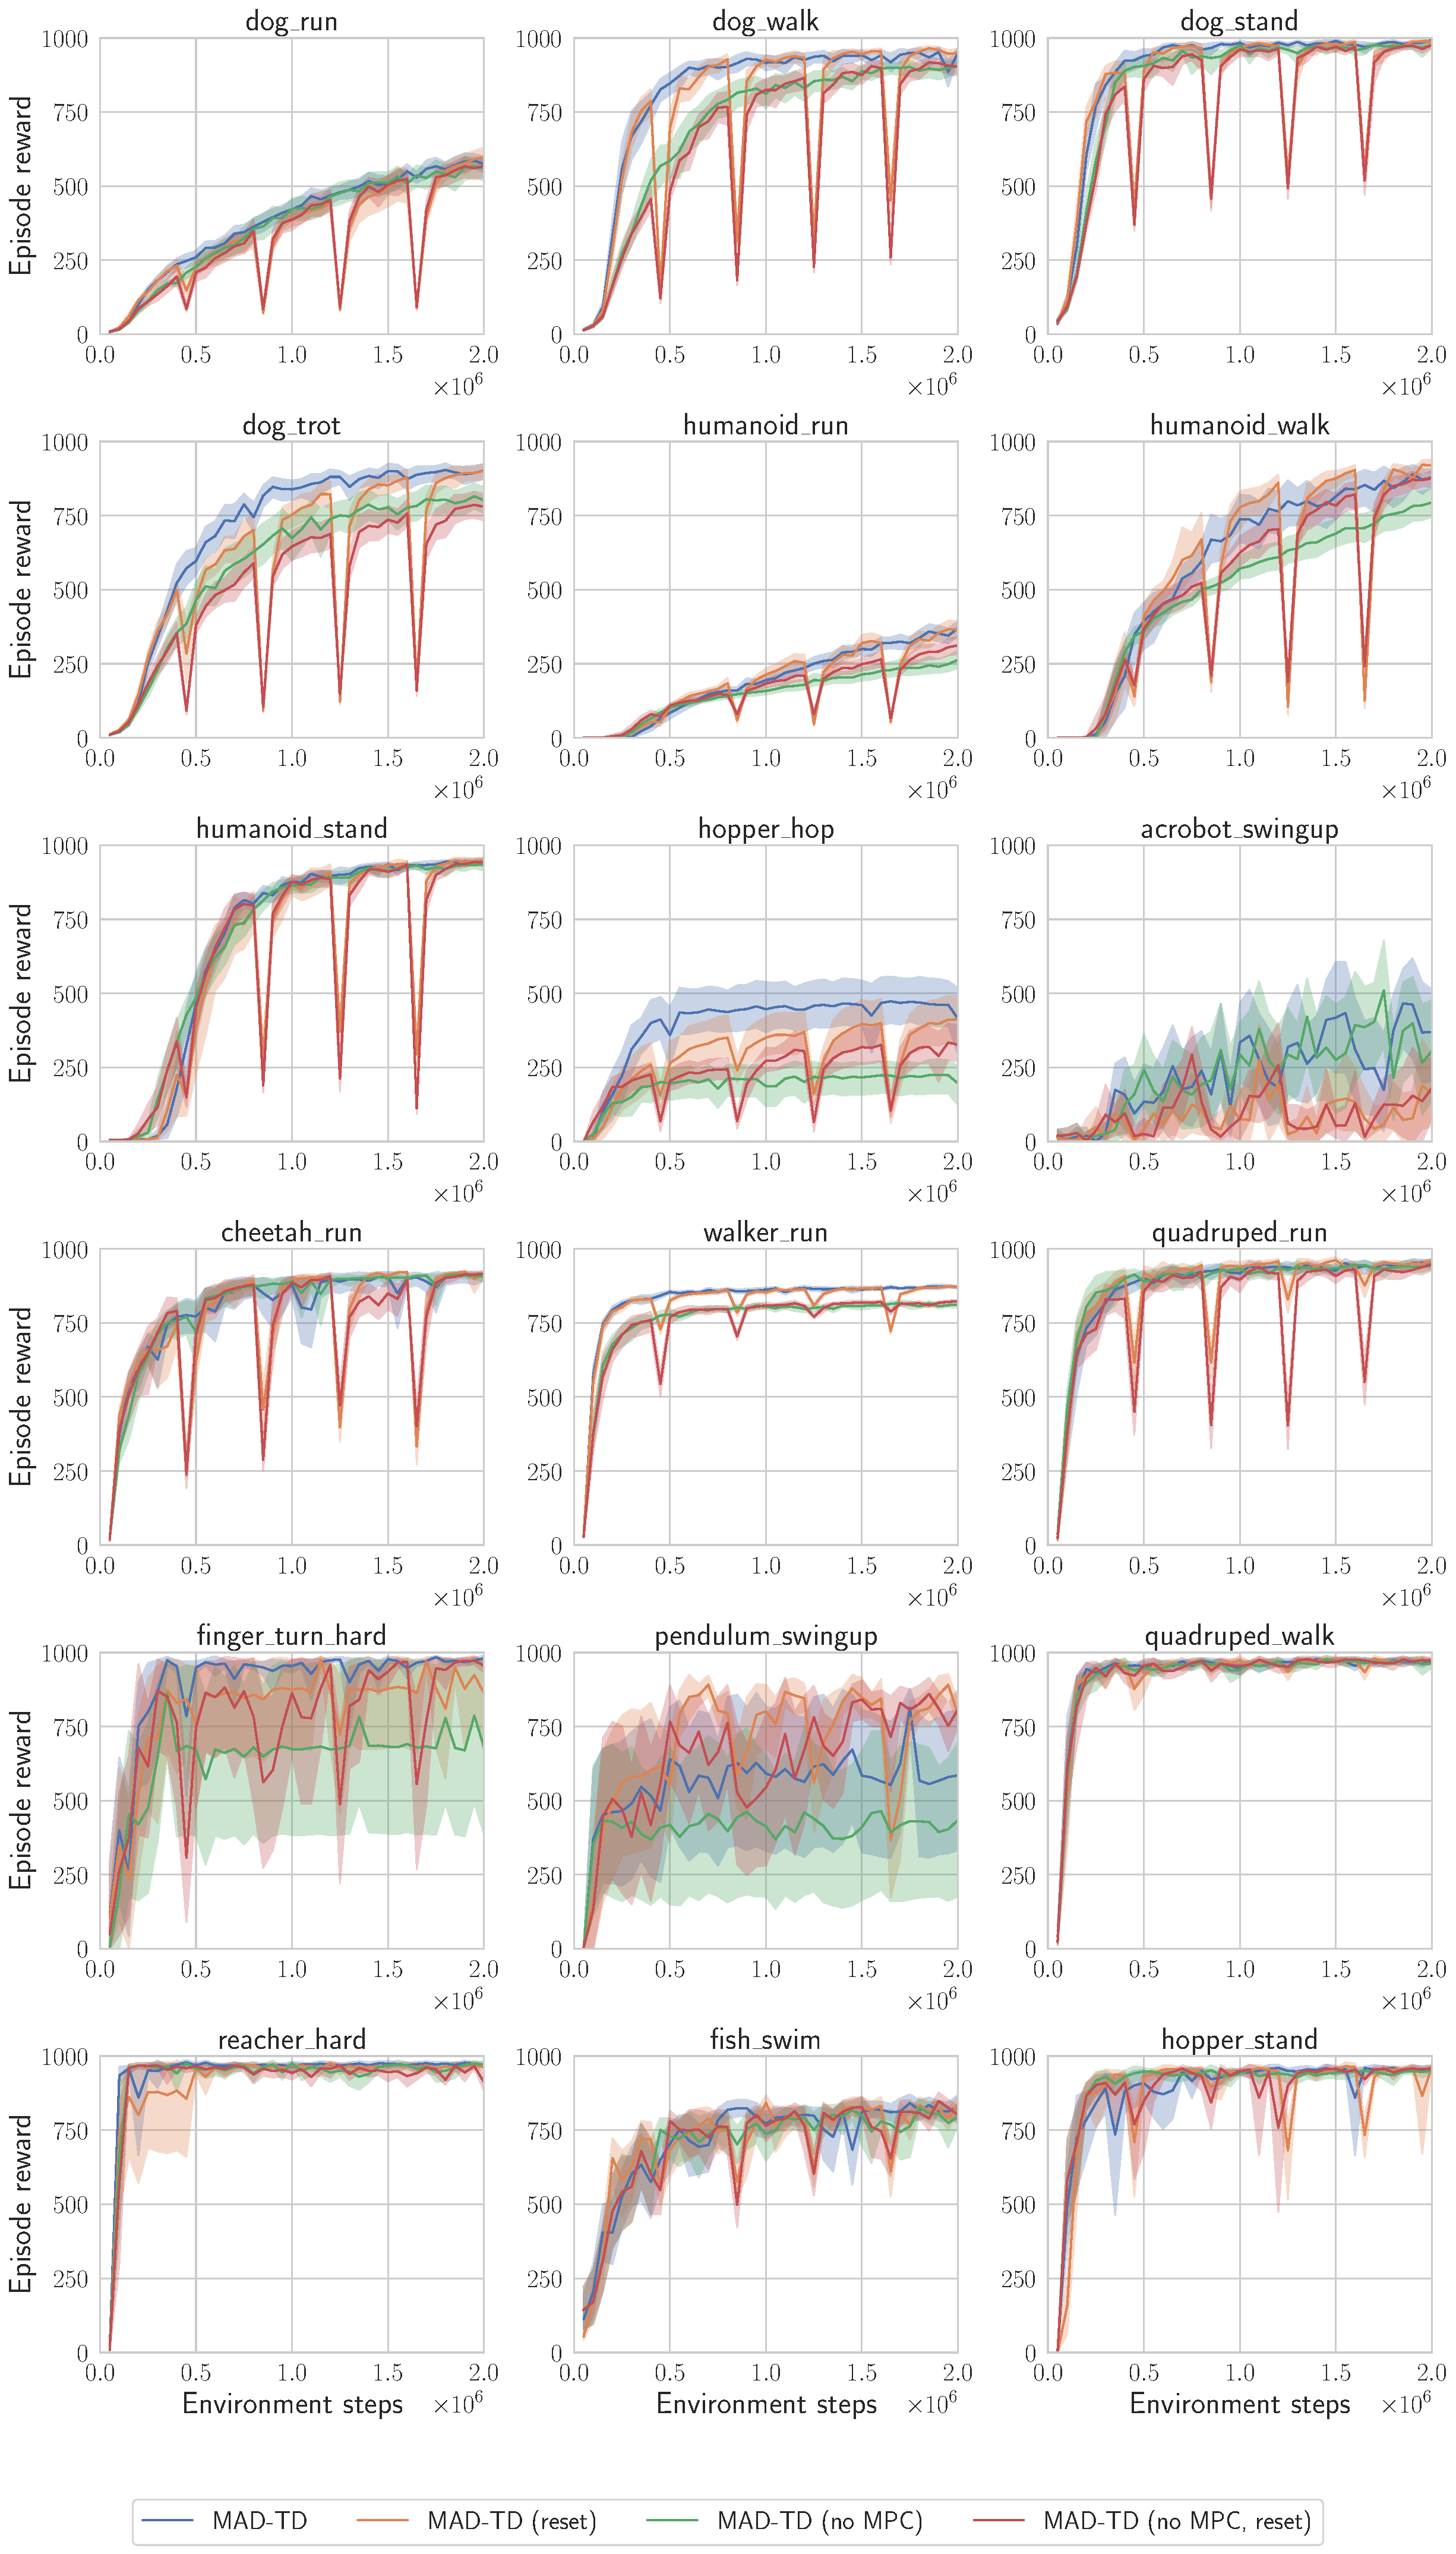
\includegraphics[width=0.8\linewidth]{figures/mad-td/mpc_reset.pdf}
    \caption{Return curves for the impact of resetting on MAD-TD with and without MPC. Without MPC, resetting can still improve the performance, but with MPC, we see no significant benefits from resetting across environments except pendulum. The hopper results highlight the importance (and danger) of the reset interval, as seemingly the reset algorithm is not able to recover ``in time'' to improve performance.}
    \label{fig:mpc_comp}
\end{figure}

% \begin{figure}
%     \centering
%     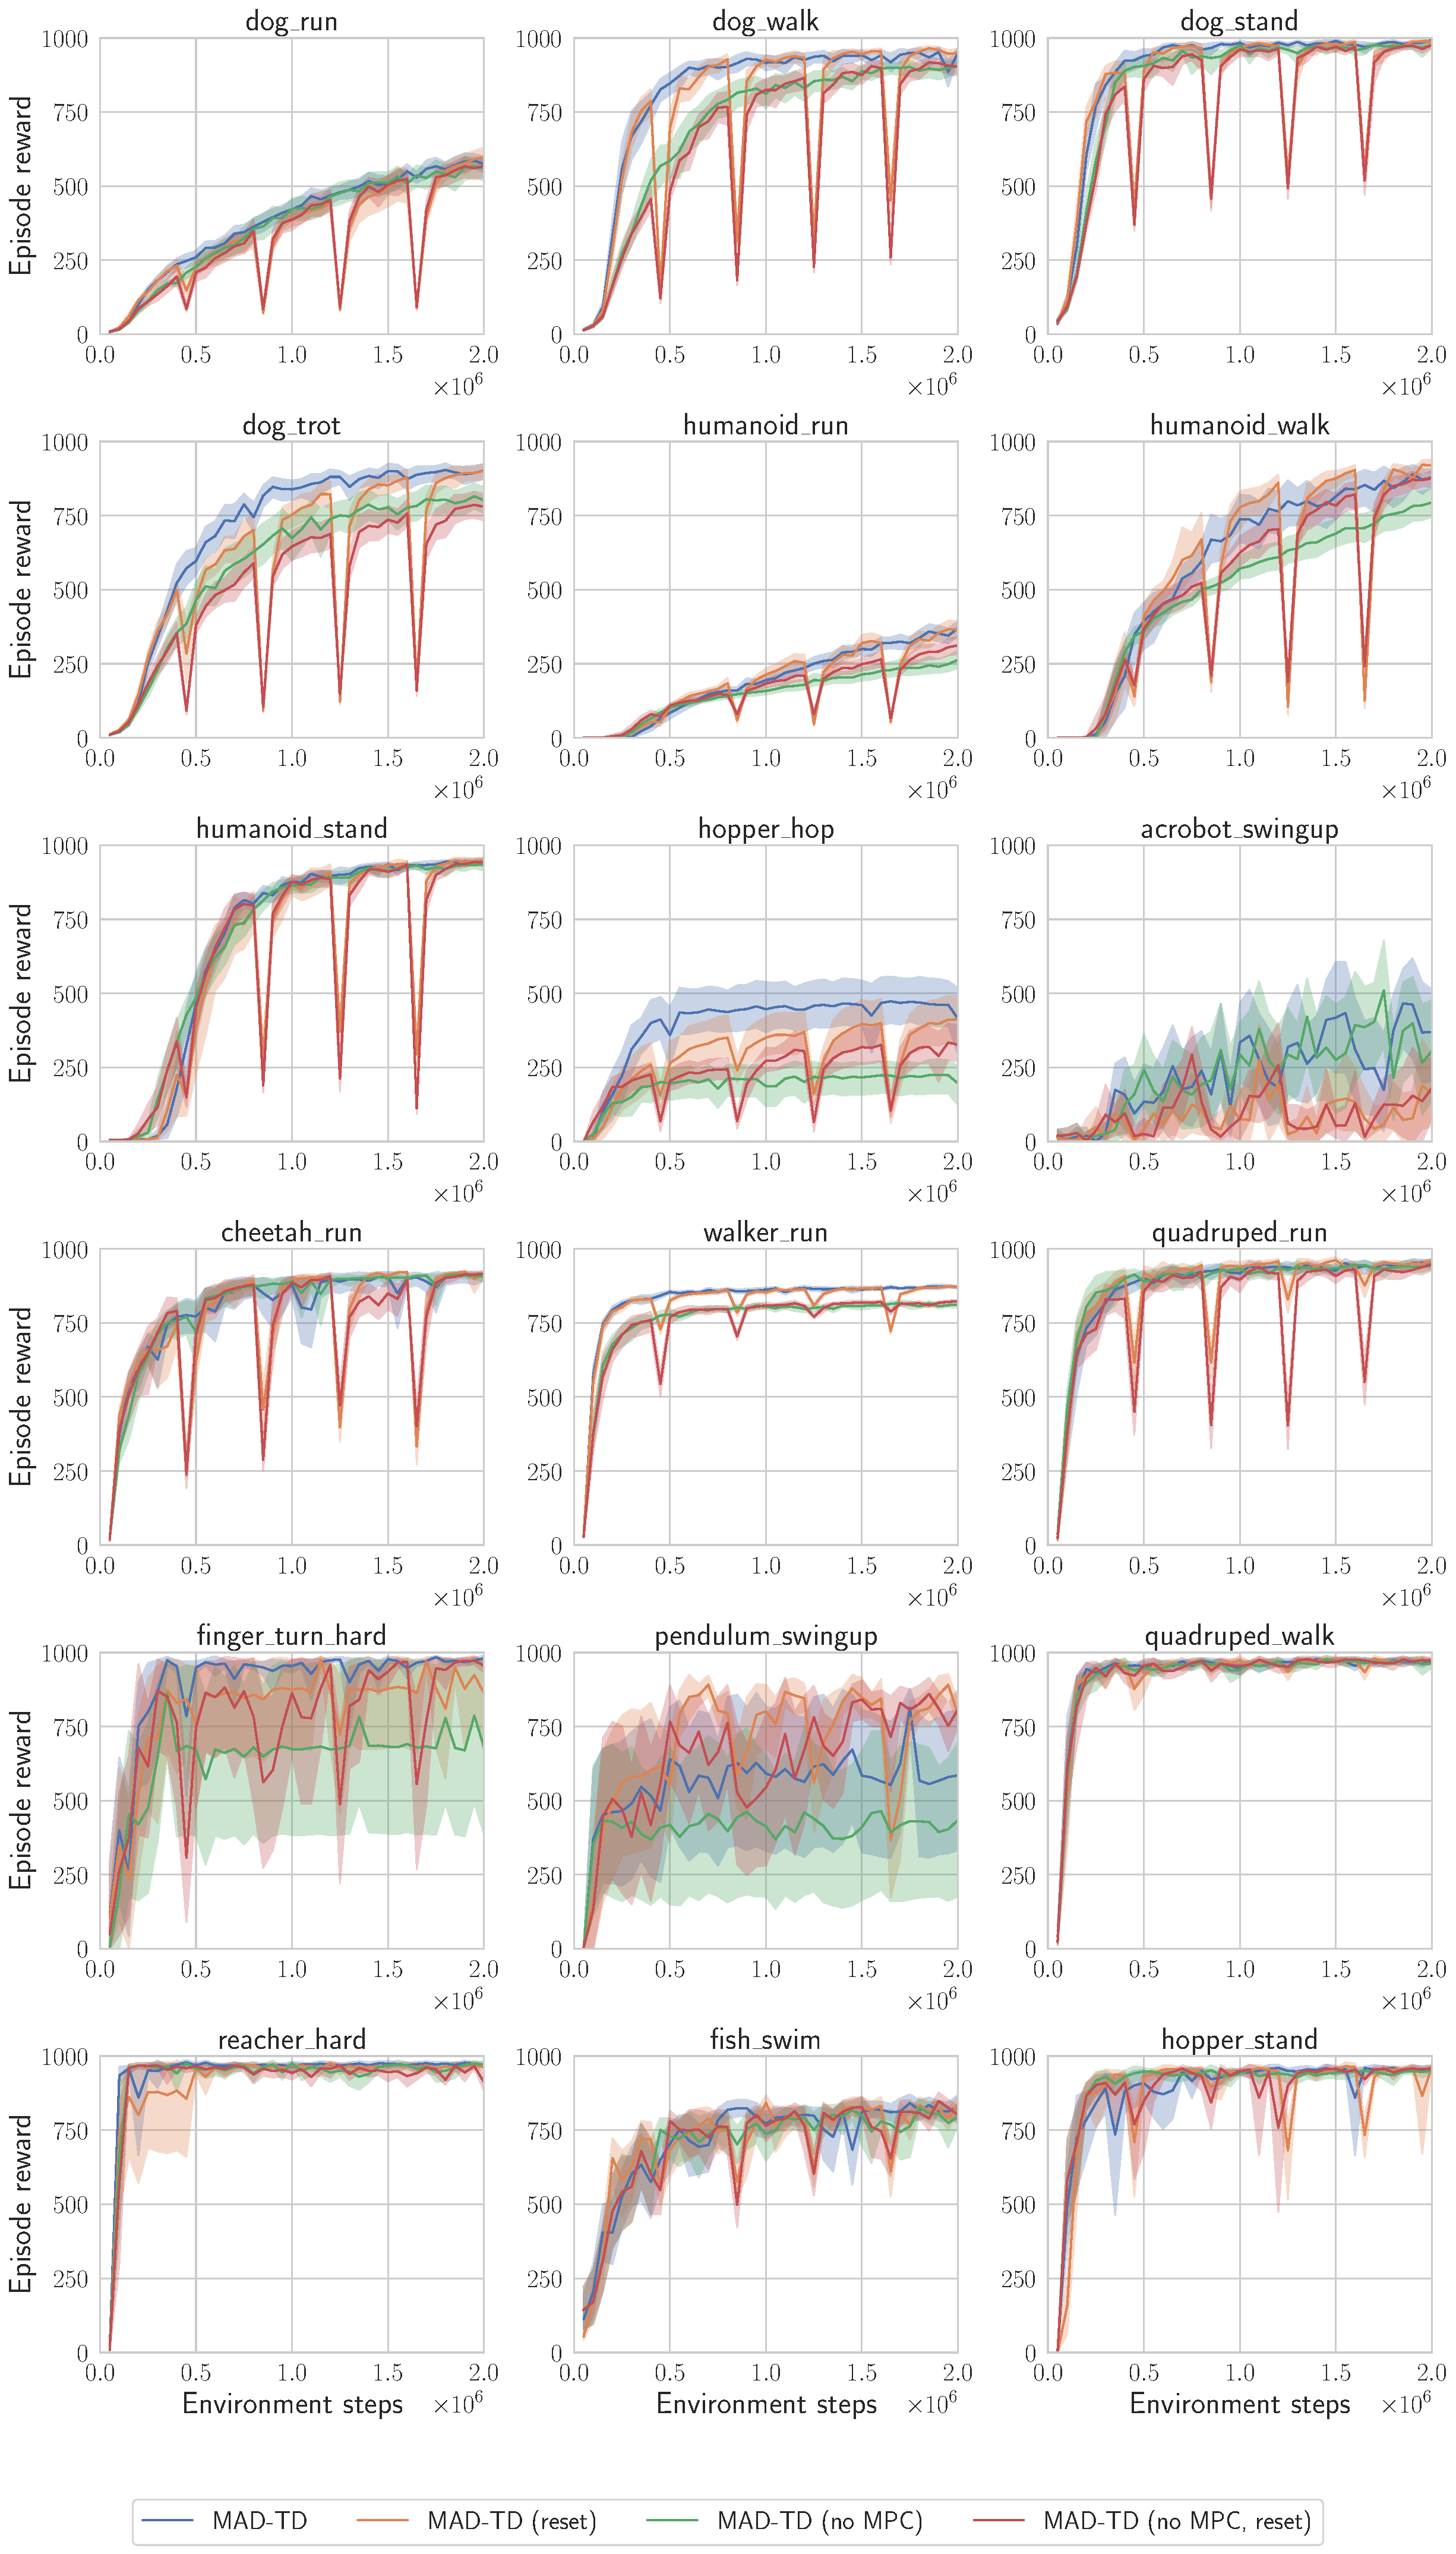
\includegraphics[width=\linewidth]{figures/mad-td/mpc_reset.pdf}
%     \caption{Placehilder for the damned trot}
%     \label{fig:enter-label}
% \end{figure}
\begin{figure}[H]
    \centering
    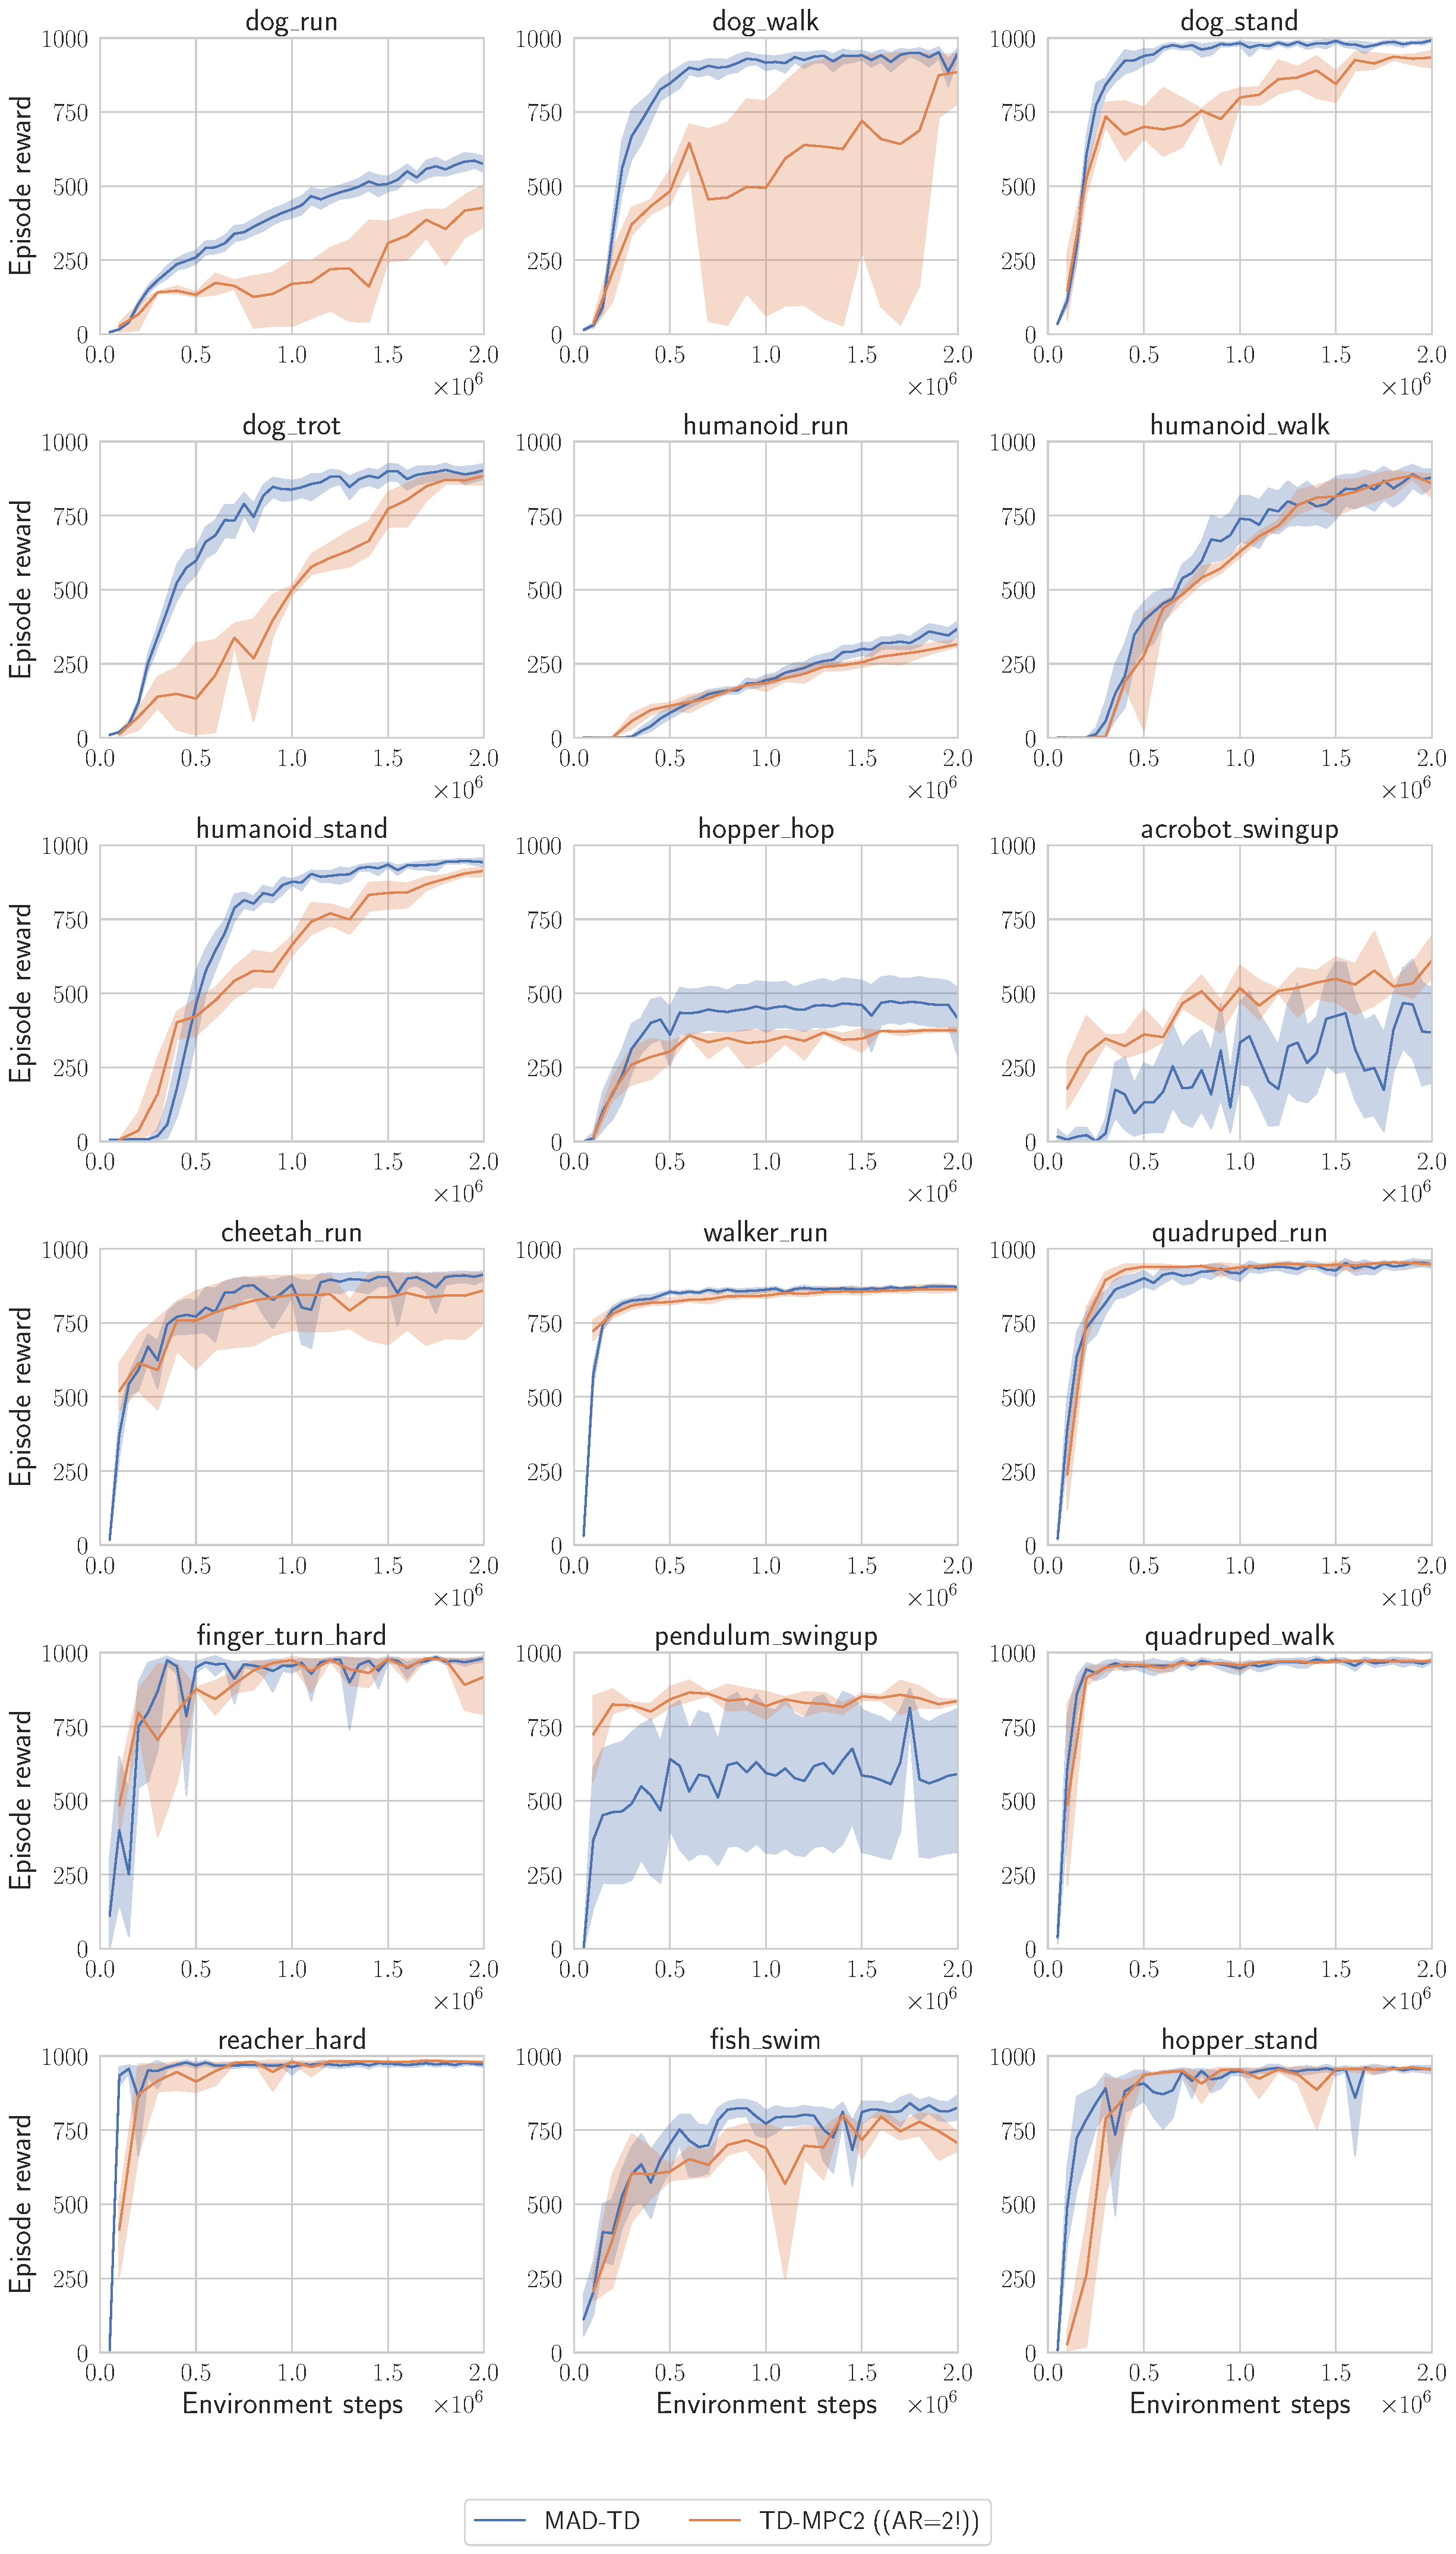
\includegraphics[width=.8\linewidth]{figures/mad-td/all_baseline_comp_rewards.pdf}
    \caption{Comparison of MAD-TD and TD-MPC2 across more environments of the DMC suite. We observe gains compared to TD-MPC2 in the hard tasks, especially in terms of early learning performance, while TD-MPC2 has advantages on the pendulum\_swingup and acrobot\_swingup tasks. These seem to be exploration and stability issues for which the longer model rollouts of TD-MPC2 seem to help.}
    \label{fig:all_baseline}
\end{figure}

\newpage
\rebuttal{
\subsection{Metaworld} \label{app:metaworld}
To broaden the basis of comparison, we compare our method to BRO and TD-MPC2 on 9 selected environments from the metaworld suite.
Results can be found in \autoref{fig:metaworld}.


Overall, we observe that our method performs strongly on tasks in which the agent has access to a dense reward, such as \emph{lever-pull} and \emph{button press}.
MAD-TD demonstrates the ability to quickly and stably bootstrap reward when available.
When exploration is a challenge, learning can take longer with MAD-TD.
Strong exploration for high-UTD algorithms is not the focus of MAD-TD and remains an open problem~\parencite{hussing2024dissecting}.
% However, when faced with sparse rewards, it can fail to learn as well.
This is consistent with our core hypothesis: high UTD learning benefits in cases where fitting a correct value function is challenging.
In tasks such as \emph{pick-place-wall} the core challenge is exploration, as the agent receives no reward signal for the majority of early training.
We therefore cannot expect high UTD learning to improve the performance in these tasks.

As pointed out, BRO and to a lesser extent TD-MPC2 have the benefit of exploring with optimism bonuses and ensembled value functions.
We removed these from our method to cleanly study the impact of model generated data.
However, improvements to exploration are mostly orthogonal to our proposed method and can be freely combined in future work.

Finally, as also shown by \textcite{nauman2024bigger}, there is a curious failure case of TD3 compared to SAC in the case of environments with sparse rewards.
In the absence of the entropy penalty form the SAC loss function, the tanh policy of TD3 tends to saturate, which can stymie exploration completely. 
This is, to the best of our knowledge, not discussed in the literature, and should be investigated in future work.
}

\begin{figure}[H]
    \centering
    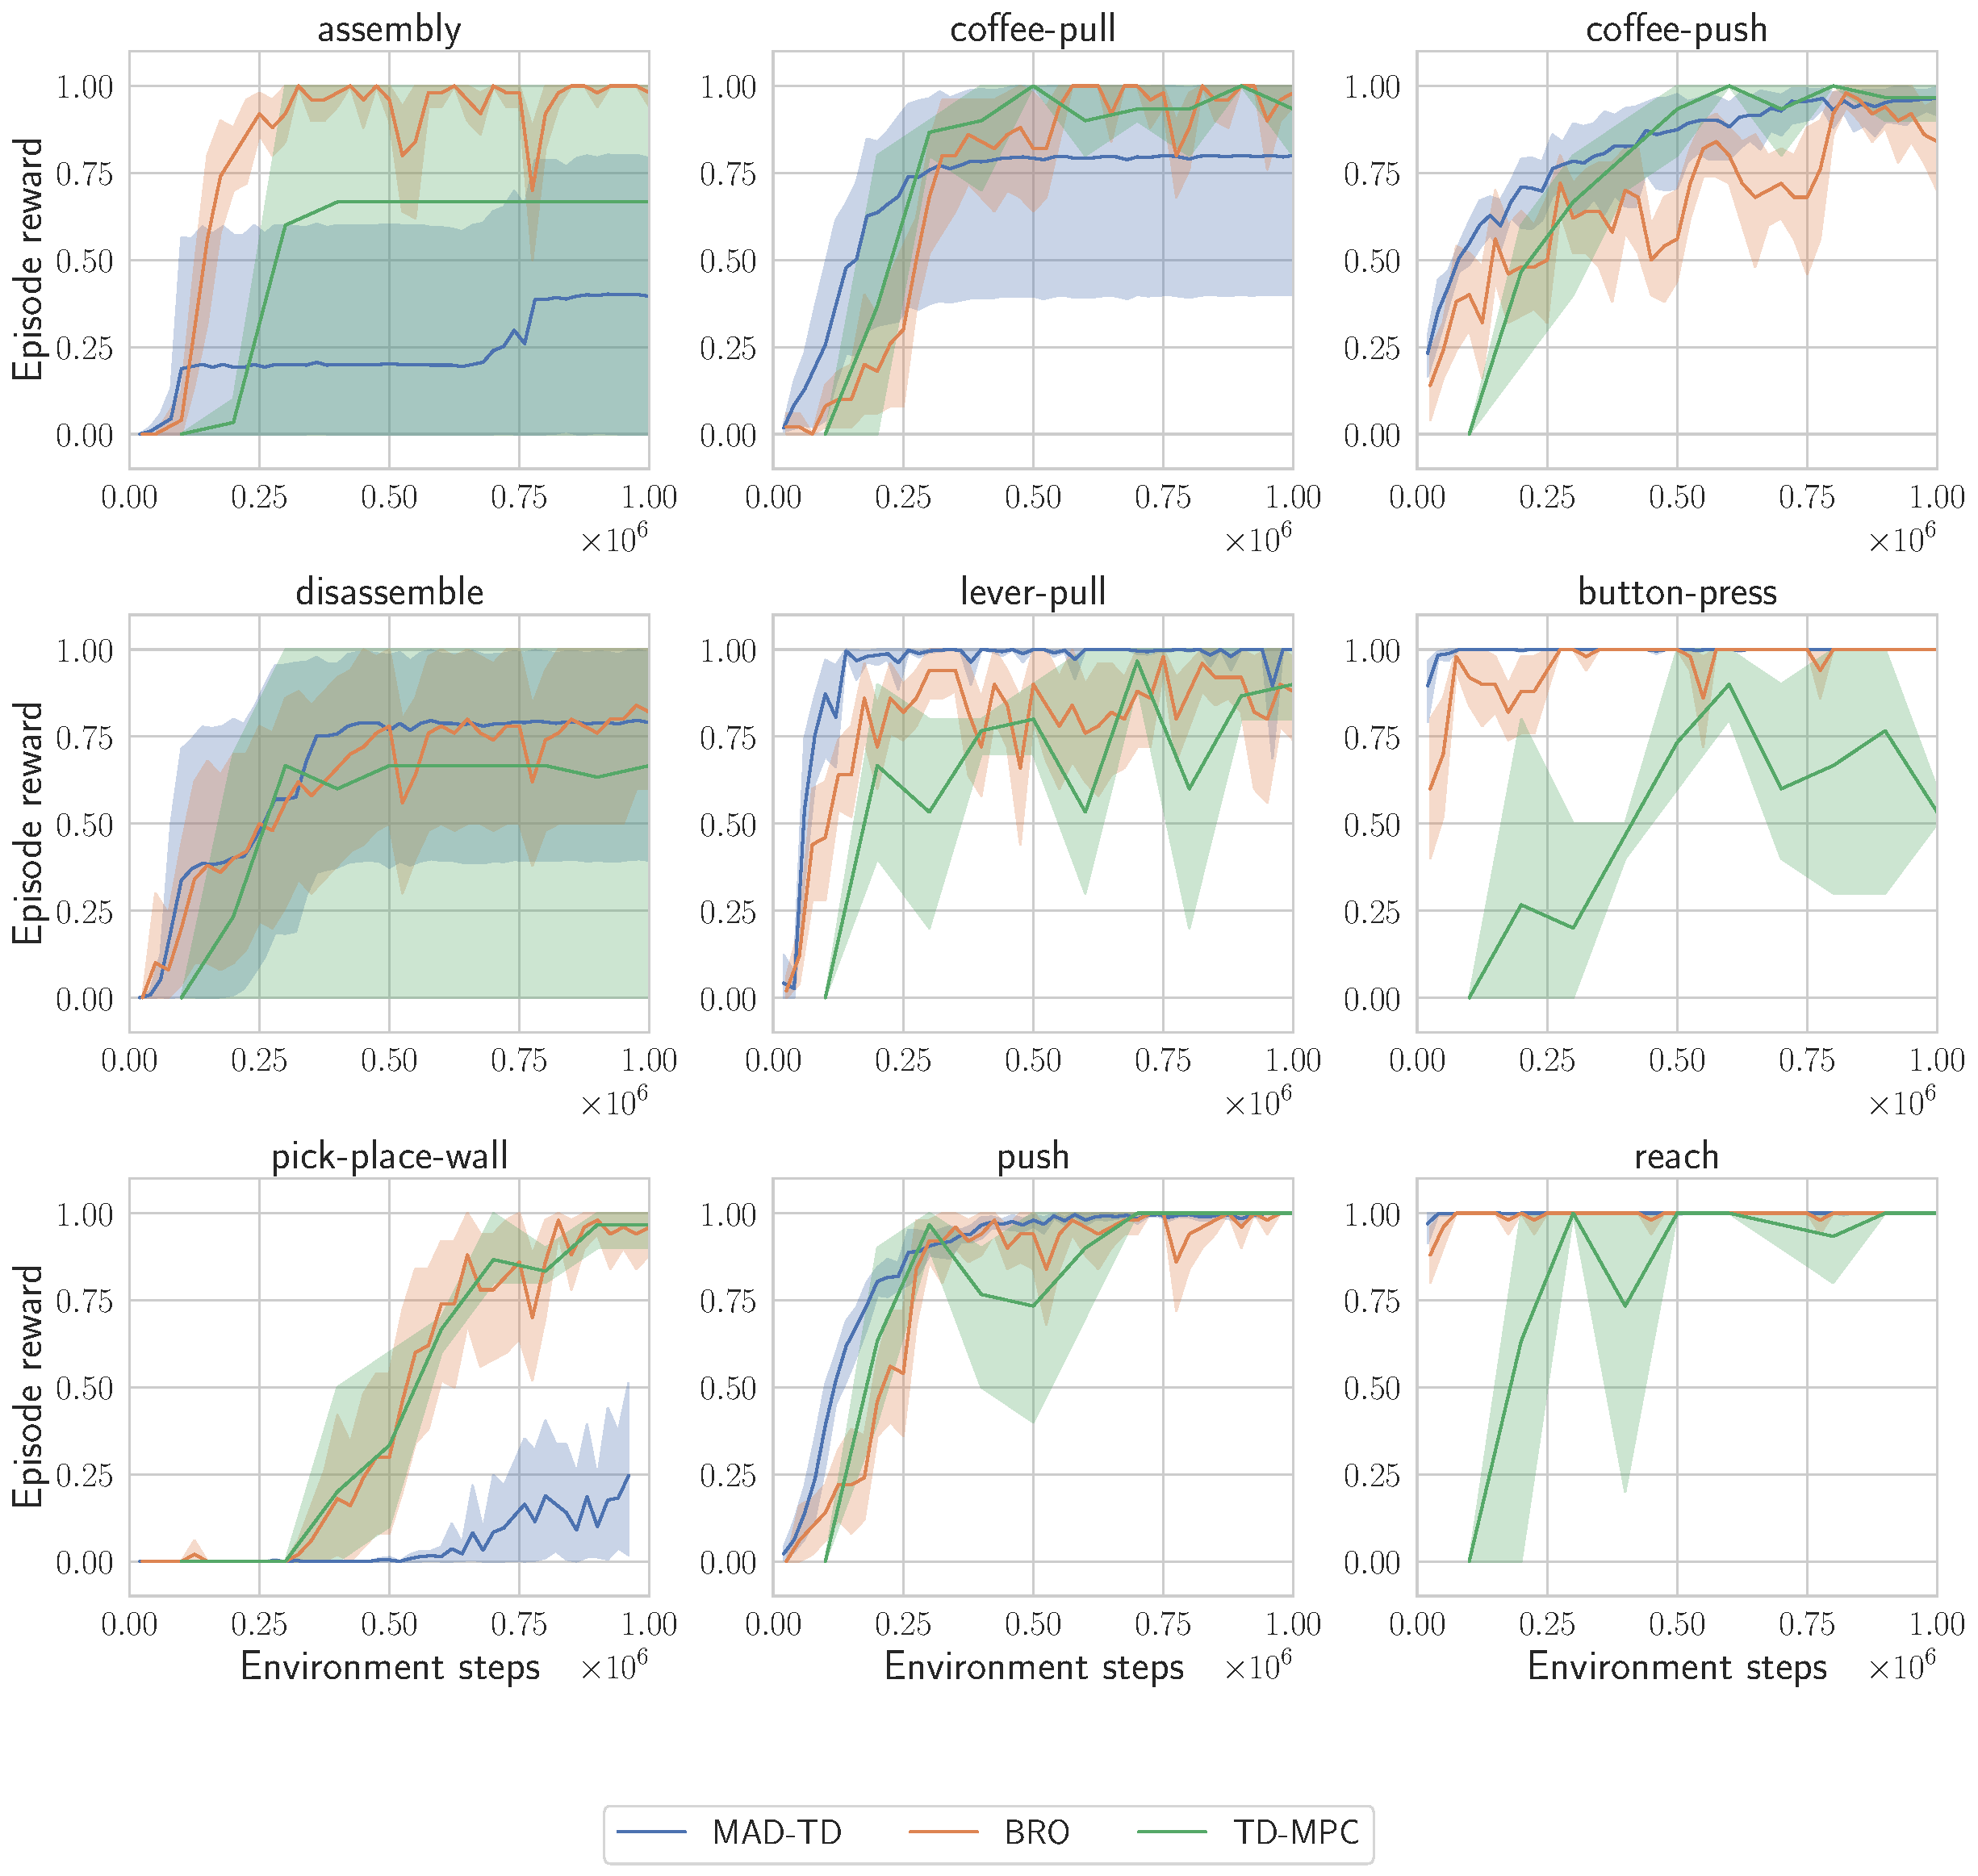
\includegraphics[width=0.8\linewidth]{figures/mad-td/metaworld.pdf}
    \caption{\rebuttal{Performance comparison on Metaworld between MAD-TD, BRO, and TD-MPC2. MAD-TD performs strongly on tasks which provide sufficient reward information to bootstrap the value function quickly, while learning more slowly on sparse reward tasks. This is consistent with the core goal of our algorithm, to stabilize and improve value function learning.}}
    \label{fig:metaworld}
\end{figure}